%%%%%%%%%%%%%%%%%%%%%%%%%%%%%%%%%%%%%%%%%%%%%%%%%%%%%%%%%%%%%%%%%%%%%%%%%%%%%%%%
%2345678901234567890123456789012345678901234567890123456789012345678901234567890
%        1         2         3         4         5         6         7         8
% THESIS CHAPTER

\chapter[Control Architecture: Simulation Results]{Control Architecture: \\ Simulation Results}
\label{chap:results}
\ifpdf
\graphicspath{{Results/Figures/PNG/}{Results/Figures/PDF/}{Results/Figures/}}
\else
\graphicspath{{Results/Figures/EPS/}{Results/Figures/}}
\fi

\begin{figure}[H]
	\centering
	\includegraphics[width=14.5cm]{scenario_whole.png}
	\caption[The Scenario with the two robot carrying the peg and the vision robot watching the hole]{The Scenario of the experiment. The two twin robots are carrying the common peg, while the third robot is watching the hole to estimate its pose.}
	\label{fig:method_uwsim}
\end{figure}

In this chapter, experimental set-up is described, and results are given and discussed. The code for the whole architecture is available at the following link:\\ \mbox{\href{https://github.com/torydebra/AUV-Coop-Assembly}{https://github.com/torydebra/AUV-Coop-Assembly}}; some details about it are discussed in section \ref{sec:controlLoop} and in appendix \ref{chap:AppendixCode}.

The scenario is made up of two I-AUV's \href{https://cirs.udg.edu/auvs-technology/auvs/girona-500-auv/}{Girona 500 AUV} underwater vehicles, each one equipped with a CSIP Robot arm5E (4 DOF arm with a parallel yaw gripper). The final goal is to successfully coordinate the robots in such a way that the peg, hold by both manipulators, is inserted correctly in the hole, fixed in the environment. In the literature, this problem is known as \textit{peg-in-hole}.\\
One robot is equipped with a force torque sensor that permits to understand forces applied on the peg, caused during the insertion phase. This information is provided to both robots. A third robot estimates the hole pose in a preliminary phase. The figure \ref{fig:method_uwsim} shows what has just been described.\\
The chosen strategy divides the problem in two phases: Hole Detection and Insertion. In the first, preliminary steps are done to detect the hole. A third robot, not used for manipulation task, is in charge to exploit computer vision algorithms to estimate the pose of the hole. Detail about this are given in section \ref{chap:vision}.
The second phase explores the problems inherent to transportation of the tool, the interaction between the peg and the hole, and the communication between the carrying agents. This is described in this chapter.

\section{Choosing the Simulator}
\label{sec:simulators}
A bit effort has been spent to choice a suitable simulator for the case. At the end, \href{http://www.irs.uji.es/uwsim/}{UWSim} [\cite{uwsim}] was chosen. It is a simulator largely used for this kind of scenarios, which visualize a virtual underwater scene. It provides a different variety of useful sensors (e.g. the used force-torque sensor and the cameras), but also others can be added. It is fully integrate in ROS, which made it really easy to use. ROS is used as simulator interface: through ROS messages, we can send commands to the robots and we can receive information from the going on test. Contact physics is implemented integrating the physics engine \href{https://pybullet.org/wordpress/}{Bullet} with \href{http://www.openscenegraph.org/}{OSG} through \href{https://github.com/mccdo/osgbullet}{OSGBullet}. To further details about how the simulation is implemented, especially the contact physics part, please refers to the documentation of the cited software. The cons in using UWSim is that the simulations is fully kinematic, so no dynamics interaction ar present. This means, for example, that velocity sent to the robot are immediately accomplished, and that we can't simulate the real physics while grasping a real object. For the scope of this thesis, this lack is not important because dynamics is not considered. Furthermore, the only needed dynamic part, i.e. how the contact between the tool and the hole affect the whole manipulator chain, can be simulated at kinematic level thanks to the information provided by the force-torque sensor, as explained in section \ref{sec:forceConsideration}.\\
To fill the lack of dynamic of UWSim, a good alternative can be \href{https://github.com/freefloating-gazebo/freefloating_gazebo}{FreeFloatingGazebo} [\cite{freeFloatingGazebo}]. In truth, this simulator is a plug-in for Gazebo and UWSim; it integrates them in order to achieve both dynamic (thanks to Gazebo) and visually realistic I-AUV simulation (thanks to UWSim). The interface used to communicate with the simulation is the same of UWSim, so ROS and its messages, which make it easy as UWSim to use. \\
This plug-in has been taken into consideration for dynamic test, that are not evaluated due to the lack of time, but can be certainly used for further works.
\href{http://gazebosim.org/}{Gazebo} is a generic simulator widely used in all robotics fields. It is the de-facto simulator for ROS. Seen its purpose, it is not a ready-to use simulator for underwater environment, and can be only a starting point to build a software to simulate this particular scenario (as it is done by FreeFloatingGazebo).\\
Also other simulators, \href{http://www.coppeliarobotics.com/index.html}{V-REP} [\cite{vrep}] and \href{https://cyberbotics.com/}{Webots} [\cite{webots}] have been taken into consideration but discarded for same \enquote{not ready-to-use} reason like Gazebo.\\
An interesting simulator is \href{https://github.com/disaster-robotics-proalertas/usv_sim_lsa}{USV simulator} [\cite{usvsim}] which takes the best from UWSim, Gazebo and FreeFloatingGazebo to implement realistic simulation. This is a really recent and in development project, and however it is focused more on surface vessels dynamics.\\

More details and comparisons are available in \cite{simComparisonCook} and \cite{usvsim}, and a schematic recap taken from \cite{usvsim} is visible in fig. \ref{fig:simComparison}.
\begin{figure}[H]
	\centering
	\includegraphics[width=14cm]{simComparison.png}
	\caption[Schematic Simulators Comparison]{Schematic recap of simulation comparison taken from \cite{usvsim}. $\times$ stands for no implemented feature; ~ $\surd\,$  for a feature that is a discrete representation of the real one; ~ $\surd\surd\,$ for a good representation of the real one. More details on how each feature is evaluated are available in the original paper.}
	\label{fig:simComparison}
\end{figure}


\section{Simulating the Firm Grasp Constraint}
\label{sec:firmGrasp}
Due to the limitation of the used simulator (explained in section \ref{sec:simulators}), some tricks have to be made. Without dynamics, simulate correctly the grasp of the peg is impossible. The simulator permits to fake the grasping with an \textit{object picker} sensor: when an object is sufficiently near to the point where this sensor is, it becomes \enquote{grasped} and it will rigidly move with the whole robot. The problem here is that we have two robots that must take the tool, so the object can't rigidly move with both, but only with the first who catch it. Furthermore, external forces applied to an object (grasped or not) can't be detected with the force-torque sensor, because, as it is implemented, it only detects forces acting on a vehicle part.\\
To solve this, a peg is modelled as additional fixed joint for each robot. In this way, each peg is rigidly attached to its own robot. Now, the problem is how to maintain the two pegs perfectly coincident during the whole mission. This is needed because the control architecture assumes a \textit{firm grasping}. This means that the end-effector does not move respect to the peg, and, consequently, the end-effectors of the robots do not move respect themselves.\\
In the simulation, collisions between the \enquote{pegs} and the hole cause them to drive apart. This is because collisions are propagated to the robots with a formula which use Jacobian (detailed in section \ref{sec:forceConsideration}). Jacobian derives from approximation of non-linear relationship, so results are not perfect. So, during the transportation, but especially during the collision propagation in the insertion phase, the two pegs distance themselves a bit. So, the control point for one robot is in a different position of what it expect, that will cause even more diverging behaviour.\\
In real scenario, firm grasp act like a \enquote{glue}: if the end effector tends to go away from the grasping point, friction acts to maintain it to the contact point. This is true for very small errors; if the cooperation performance is bad, the common tool falls down or something breaks.\\
In the simulation, to fake the firm grasp, an additional routine is implemented: it simply calculates the distance between the two peg, and generates robot velocities to zeroing this distance. It is important to note that this is an help that we would have also in real scenario, as explained before. The only difference is that, in real scenario, if the errors are too big the end-effector begins to slip, and it will never return to its original grasping point. In this case, it returns always to the initial point. \\
The velocity generates by this routine are not so big to hide bad cooperation; so the tests are suitable to evaluate the proposed architecture, and to simulate real situation.

\section{Collision Propagation}
\label{sec:forceConsideration}
When a robot interacts with the environment, each contact generates forces on it. Mission about assembling objects can't be studied in a properly manner without some considerations about these forces. In a peg-in-hole Mission, collisions between the peg and the hole will be transferred through the whole kinematic chain until the floating base, causing disturbance to the whole robotic system. Thus, it is necessary to simulate these behaviours.\\ 

Let us define $\boldsymbol{f} \in \mathbb{R}^3$ and $\boldsymbol{m} \in \mathbb{R}^3$ as:
\begin{equation}
\boldsymbol{f} = \begin{bmatrix}f_x \\ f_y \\ f_z\end{bmatrix} \qquad
\boldsymbol{m} = \begin{bmatrix}m_x \\ m_y \\ m_z\end{bmatrix}
\end{equation}
being the $\boldsymbol{f}$ and $\boldsymbol{m}$ the resultant forces and torques (projected on the tool frame $ \langle t \rangle $) of all the forces and torques acting on the tool. These disturbances generate joint velocities $ \dot{\boldsymbol{y}}_{\delta} \in \mathbb{R}^l$ [\cite{bookSiciliano}]:
\begin{equation}
	\label{eq:forTor}
	\dot{\boldsymbol{y}}_{\delta} \triangleq 
	\begin{bmatrix} \dot{\boldsymbol{q}}_{\delta} \\ \boldsymbol{v_1}_{\delta} \\ \boldsymbol{v_2}_{\delta} \end{bmatrix}
	= \begin{bmatrix} k_q \\ k_{v1} \\ k_{v2} \end{bmatrix} \, \begin{bmatrix}\;(^{lin}\boldsymbol{J}_t)^T \boldsymbol{f} + \;(^{ang}\boldsymbol{J}_t)^T \boldsymbol{m}\end{bmatrix} 
	\qquad 0 < k_q, k_{v1}, k_{v2} < 1 
\end{equation}
where $J_t$ is the Jacobian which express how Cartesian velocity $\dot{\boldsymbol{x}}_t$ of the tool are affected by the system velocity vector  $\dot{\boldsymbol{y}}$; $lin, ang$ superscripts refer to \textit{linear} (top three rows) and \textit{angular} (bottom three rows) parts of $J_t$; $\dot{\boldsymbol{q}}_{\delta}$ is the velocity vector for joints caused by the collisions; $\boldsymbol{v_1}_{\delta}$ and $\boldsymbol{v_2}_{\delta}$  are the linear velocity and angular velocity of vehicle caused by the collisions; $k_q, k_{v1}, k_{v2}$ are positive gains smaller than $1$, in general different from each other  because we are considering different types of velocities.\\


\section{Assumptions}
It is important to detail the assumptions made during the simulation. Some problems, that are necessary to be taken into account in a real environment, are not explored. This is necessary due to the difficulty of the particular scenario chosen. In this section, the more important assumptions are summarized.

\begin{itemize}
	\item Simulation is only kinematic. This implies, for example, that the commanded velocity to the vehicle and the arm are accomplished \textit{instantaneously} and \textit{perfectly}. Another implication is that the movements of arm and of the vehicle don't influence each other at all. The only \enquote{dynamic} implemented is caused by collision between the peg and the hole, which \enquote{transfer} the forces and torques acting on the peg along the whole arm (as described in \ref{sec:forceConsideration}).
	
	\item The initial configuration shows the peg already \textit{correctly} grasped by both robots. Also, the position of where the end effector have grasped the tool and the peg dimensions are known. This implies that relative position between each robot and peg's tip is \textit{perfectly} known. Such a initial configuration has been chosen because the grasping phase and problems arising during cooperative transportation have been explored in others already cited project like MARIS and ROBUST (e.g in the work \cite{IntroMaris2}) and they are also part of different studies of the on-going project TWINBOT.
	
	
	\item Pose (linear and angular displacement) of the two carrying robots and of the vision robot respect a common inertial frame (denoted as \textit{w} - \textit{world} in the whole thesis) is known. In real situation, the pose underwater is always an issue and it is never really precise. Good precision can be provided, for example, after some works in mapping the seafloor, which will provide a common reference point somewhere. Note that it is not important know the pose of the robot respect to a point above the water surface (that can be done thanks to information shared with surface vessels, for example as explored the WiMUST project [\cite{wimust}]). The important thing is to know relative pose of the robots to a common node, that can also be underwater. This is needed to make the vision robot share correctly the estimated hole's pose with the carrying robots.
	
	\item No real communication issues between the two carrying robot are taken into account. The presence of water puts important issues in real situation: \textit{full-duplex} communication (i.e. sharing data \textit{at the same time}) is impossible, and, in general, there is a lower bandwidth than in the air. Some experiments in simulated environment with different methods of underwater communication are detailed in \cite{IntroMaris2}.\\
	However, these issues are considered by the cooperative scheme (explained in section \ref{sec:coopScheme}); in fact it permits to exchange very few information between the two carrying agents.
	
	\item The two robots firmly grasp the peg. There is no sliding caused by robot movements. This point is detailed in section \ref{sec:firmGrasp}.
	
	\item During the insertion phase, the architecture resolve alignment errors \textit{only if} the peg is inside the hole. If the peg touches the external hole surface, no routines are implemented to deal with the problem of \textit{looking} for the hole on the surface.
	
	\item The sensor is positioned on the tip of the peg, and it provides forces and torques caused by contacts with the whole peg. This would obviously not possible in real applications. In real scenario the sensor is usually put on the wrist and provide forces respect to this point. However, we could project the force-torque sensor information on another frame, if we know the relative pose. This assumption is also necessary because the chosen simulator can give force-torque information only on the part where the sensor is positioned.\\
	Also, both robots have access to the sensor data, without uncertainties (except numerical errors due to how almost all physics engines compute collisions, that it is done with approximations to improve the performance).
	
	%todo altre? 
\end{itemize}

\noindent Others assumptions, more related to the vision part, are detailed in section \ref{sec:visioAssumption}.

\section{Control Loop}
\label{sec:controlLoop}
\begin{figure}[H]
	\centering
	\includegraphics[width=12cm]{flowScheme.png}	
	\caption[Flow Scheme Control Loop]{A flow scheme showing the main step of a single control loop for the robots and for the coordinator. Blocks at the same horizontal level are executed at the same time. Arrows indicate sharing of data between blocks of different nodes. Note here that the vision robot is not considered.}
	\label{fig:flowScheme}
\end{figure}

This section is made to give a better idea on how the control architecture works.\\
The Vision Robot, which job is to estimate the hole pose, acts in a preliminary phase. It \textit{tracks} the hole, thanks to stereo-cameras, and it sends the estimated pose to the two carrying robots (and to the Coordinator). Due to its nature, no complicated control is implemented for this agent: when the pose is sent, we simply move it away from the hole with keyboard (like a ROV) to not interfere with the insertion mission. This part is described in Chapter \ref{chap:vision}.\\

The two carrying robots are completely autonomous: as soon they get the hole pose, they start, \textit{without user intervention}, the main mission. There are three nodes: the two Robots (\textit{A} and \textit{B}) and the Coordinator. The latter is not a real \textit{physical} agent: it is only a software routine. So, it can be physically inside one robot, let's say Robot A. In this way, communication issues (due to the underwater scenario) happen only between the two robots, and not among all the three nodes.\\
Initially, the Agent A, the Agent B and the Coordinator synchronize themselves, i.e. each one waits that the other two are ready. After this initialization phase, the normal routine starts, as can be seen in figure \ref{fig:flowScheme}, where the main instructions of the control loop are depicted.
\begin{itemize}
	\item At the beginning of the control loop, each node gets the updated simulation state, e.g. pose of the robots, pose of the tool, information from force-torque sensor, and so on.
	
	\item The Coordinator, which (as said previously and without loss of generality) is a software routine inside the Robot A, modifies the goal's linear position (as explained in \ref{sec:changeGoal}), if some forces are detected. If the goal is updated, the two Agents get this new information.
	
	\item In the third block's row, the Robots run the first TPIK procedure. Then, they send the necessary data to the Coordinator, which computes the cooperative velocities and sends them back to the robots. Finally, the two Agents run another two TPIK procedures, one for the cooperation and the other for the vehicle-arm coordination. This routines are described in Section \ref{sec:armVehScheme} and Section \ref{sec:coopScheme}. In all the TPIK procedure, the Force-Torque objective (Section \ref{sec:forceTask}) is used.
	
	\item At the end, the two Agents send the outputs (i.e., the system velocity vectors) to the simulation.
	
	\item Before sending the velocities to the \enquote{real} simulation, some disturbances must be added to the commanded system velocity vectors. For the Robot A, this means adding effects of collisions between the peg and the hole (Section \ref{sec:forceConsideration}). Instead, for the Robot B, effects of the firm grasp constraint are added (Section \ref{sec:firmGrasp}).
	
	\item After the simulation performs a step, the routine starts again.
	
\end{itemize}
\vspace{20px}
It can be noticed that the two added physical interactions (collisions and firm grasping constraint) are added only for one robot (A and B, respectively) and not for both.\\
This is done to not add simulation errors that can occur, and that would not happen in real scenario. For example, in real situation there are not two coincident pegs (as in this simulation) and so they can't really distinguish themselves. Putting the firm grasp constraint only on one robot helps to reduce disturbances that in real scenario are not present. Also, it is sufficient to fake a real firm grasping.\\
About the collisions, they affect, \textit{directly}, only the first agent. In truth, they also affect the other one, \textit{indirectly}, because the latter is \textit{dragged} by the firm grasp constraint. So, practically, collisions affect the behaviours of both agents.\\
It is important to notice that these physical interactions do not hide control problems: if the control is setted badly, the whole mission fails (e.g. the two peg diverge and/or compenetrate visibly with the hole).\\
%%%%
Another thing to notice is that, when the Force-Torque objective (Section \ref{sec:forceTask}) is used, both Robots need the sensor data. Being the force-torque sensor only on Robot A, this means that additional communication between Robot A and Robot B is needed. As known, underwater transmission is difficult and slow, and the general amount of the exchanged data should be keep as small as possible (from this problem it derives the used coordination policy).\\ 
An alternative can be to use another sensor on the Robot B. The problem following this direction could be that different sensors give not exactly same data. So, the two robots run each TPIK with different information. This problem is not explored here.\\
Another solution can be simply to avoid using this objective: it would decrease the performance of the mission (as we will see later) but results are good anyway.\\
It must be noticed that also to update the goal additional information has to be exchanged between the two robots. 

\section{Results}
\label{sec:resultNoVisio}
\begin{figure}[H]
	\centering
	\includegraphics[width=10cm]{scenario_onlyTwin.png}
	\includegraphics[width=10cm]{scenario_onlyTwin2.png}
	
	\caption[Scenario for tests without the vision part]{Two different points of view of the scenario for the results presented in this section. The pose estimation with vision is neglected here.}
	\label{fig:onlyTwin_uwsim}
\end{figure}

The first experiments do not take into consideration the vision part, to have a hole's pose error arbitrarily settable to discuss the performance of the methods used. The figure \ref{fig:onlyTwin_uwsim} shows the robots initial position. Below, a list of important details about the simulations:
\begin{itemize}
	\item The \textbf{Peg} is a six meters long cylinder, with a diameter of 0.10 meters.
	\item The \textbf{Hole} is a cylindrical cavity with a diameter of 0.14 meters
	\item The initial position of the agents is near the hole: the peg's tip is almost aligned perfectly to the hole, and it is at almost 0.44 meters from it. To be precise, the vector from peg's tip to the hole has components : $[0.441, -0.008, -0.018]$ where $x$-component is along the length of the peg, $y$-component lies on the tip's surface and it points to the left, and $z$-component points downward (as in fig. \ref{fig:scenario_frames}). Considering the peg's tip frame described by these components, the orientation from the peg's tip frame to the hole frame is described by these Euler angles: $[0, 0, 1.942]$ (\textit{roll, pitch, yaw}, in degrees).
	\item The \textbf{goal} is to drive the peg inside the hole with a depth of 0.2 meters.
	\item All the vectors displayed in the plots are projected in the world frame (which orientation is visible in fig. \ref{fig:scenario_frames}).
\end{itemize}
\begin{figure}[H]
	\centering
	\includegraphics[width=12cm]{scenario_framesCrop.png}	
	\caption[Scenario with the main frames]{Detail of a screenshot where the main frames are drawn. The world frame is present only to clarify its orientation; its origin is not in that point. For the hole frame, the $x$-axis goes inside the cavity. The goal frame $\langle g \rangle$ has the same orientation of the hole frame, and it is shifted of 0.2 meters in the direction of hole's $x$-axis.}
	\label{fig:scenario_frames}
\end{figure}

In the following results, only a few plots (fig. \ref{fig:expWithVisioVel} and fig. \ref{fig:expWithVisioVelTool}) are related to the cooperation scheme of section \ref{sec:coopScheme}, and no long discussions are made for them. This choice has been made because no robot has difficulty in tracking the ideal common tool velocity $\dot{\boldsymbol{x}}_t\,$, so no very interesting plot occurs. Experimental results about this particular scheme used can be found in \cite{IntroMaris2} and \cite{tesiWander}.\\

The focus of the results is on the implemented methods for helping the insertion phase: the Force-Torque objective (section \ref{sec:forceTask}) and the Change Goal routine (section \ref{sec:changeGoal}). Further outcomes are presented about the added simulation procedures: the Firm Grasp constraint (section \ref{sec:firmGrasp}) and the Collision propagation (section \ref{sec:forceConsideration}). These last two extensions are important to improve the simulation in an otherwise pure-kinematic scenario.

\subsection{Perfectly known Hole's pose}
In the first experiment, the hole's pose and the goal frame $\langle g \rangle$ are known without uncertainties. The plots of figure \ref{fig:noErrorPlots} show how the forces and torques act on the peg, the converging positional error from the goal to the peg's tip, the tool velocities generated by the collisions, and the tool velocities caused by the firm grasp constraint.
\vspace{20px}
\begin{figure}[H]
	\centering
	\textbf{Perfectly known Hole's pose}\\
	\vspace{8px}
	\centerline{
		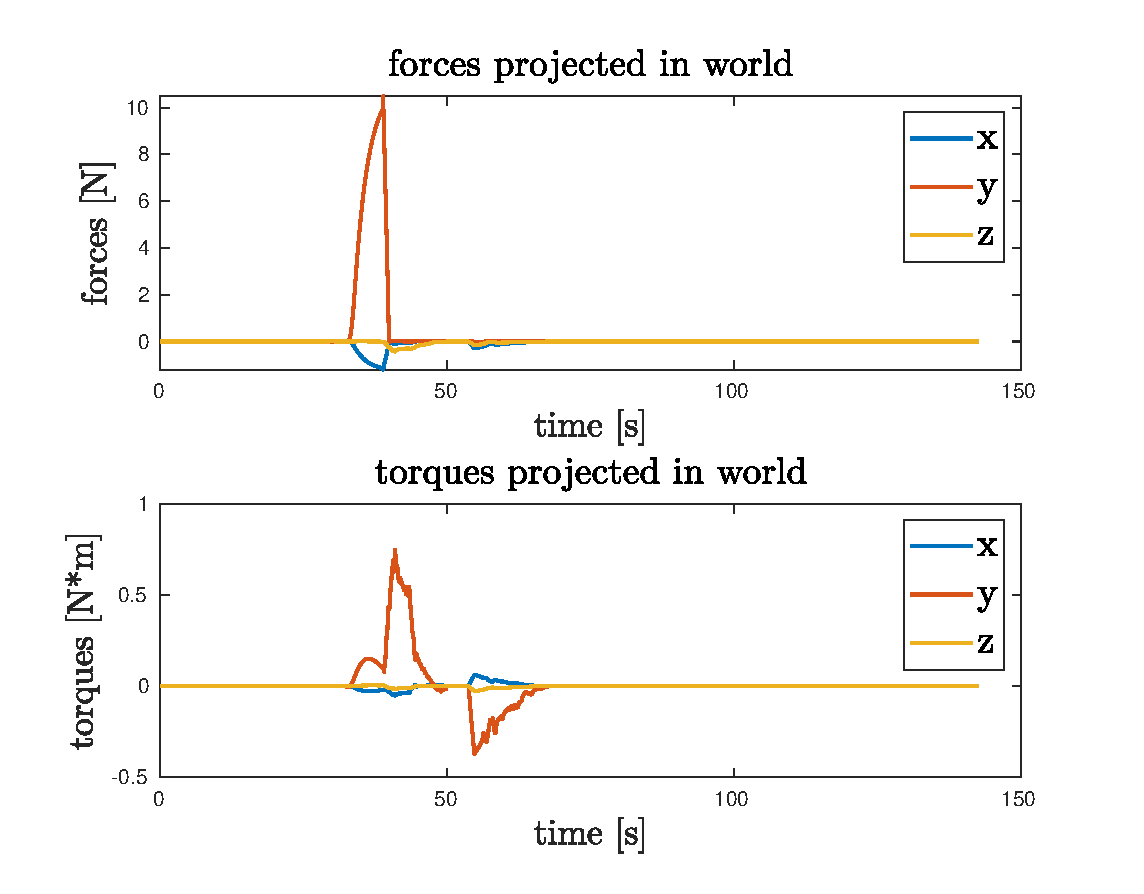
\includegraphics[width=8.8cm]{NOERROR/forces.eps}
		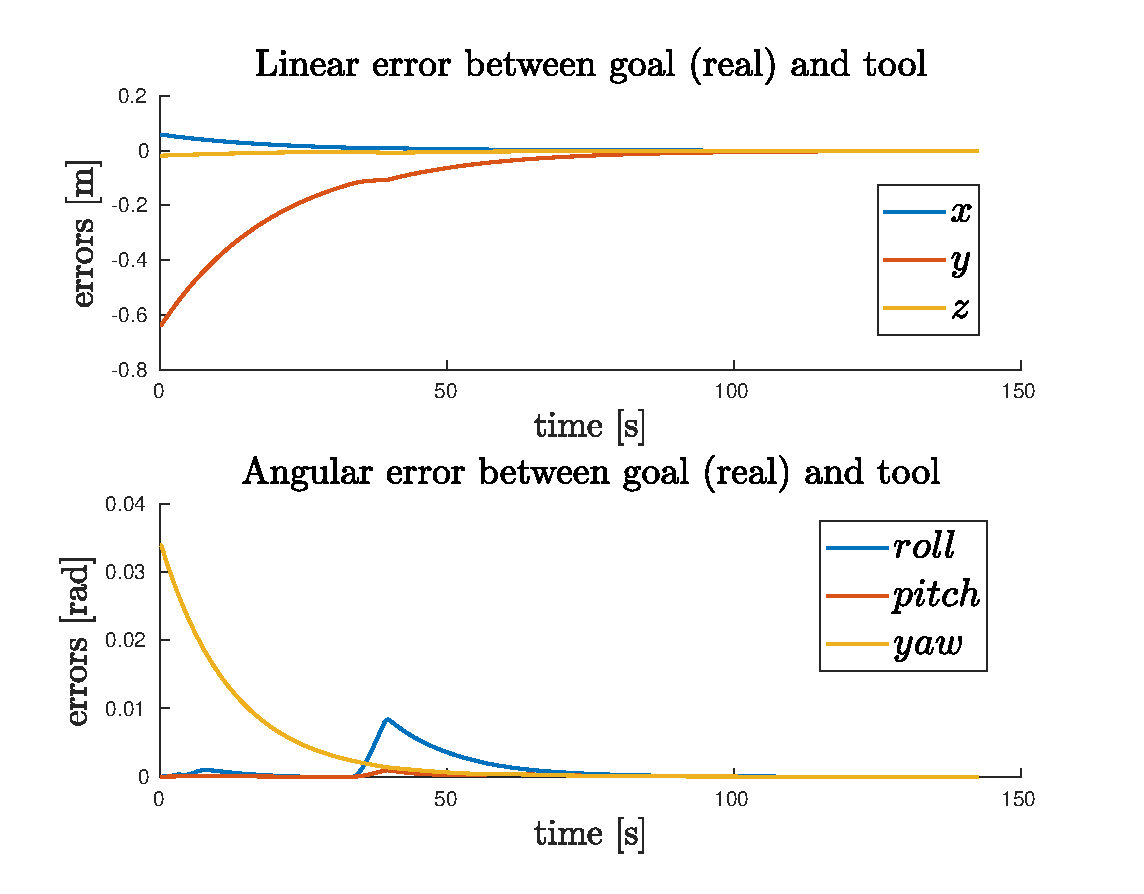
\includegraphics[width=8.8cm]{NOERROR/error.eps}
	}
	\vspace{6px}
	\centerline{
		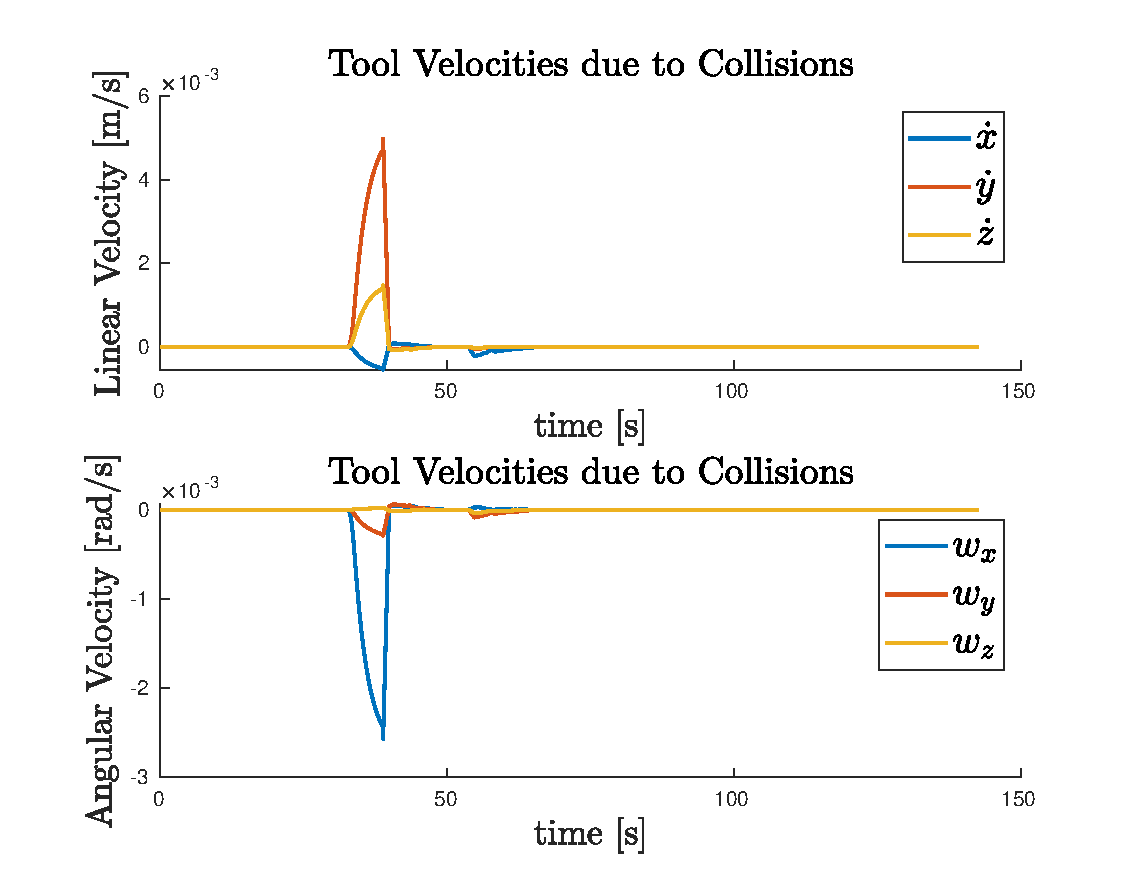
\includegraphics[width=8.8cm]{NOERROR/collisions.eps}
		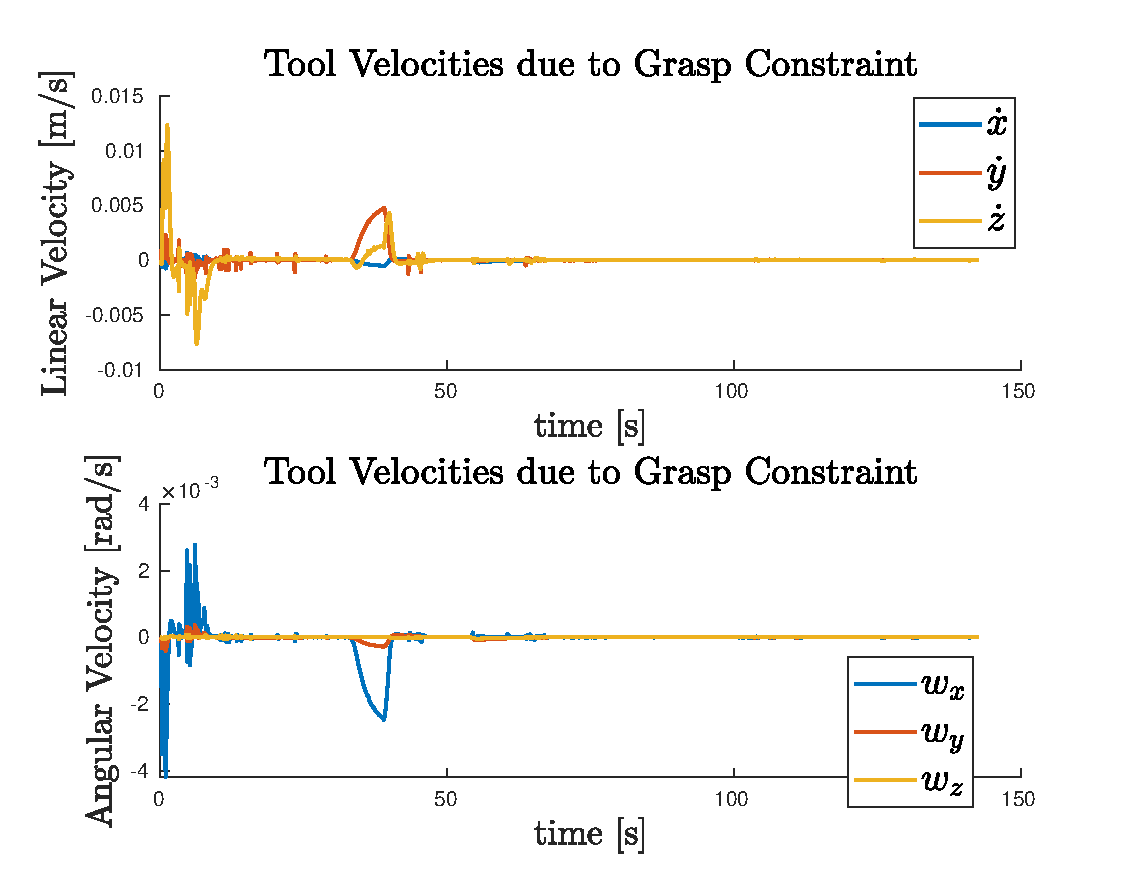
\includegraphics[width=8.8cm]{NOERROR/grasp.eps}
	}
\end{figure}
\captionof{figure}[Plots with Perfectly known Hole's pose]{The results with the hole's pose known without errors. The upper left plot shows the forces and torques acting on the whole peg: they are the components of the total resultants projected on world. The high peak in $y$ is due to the first contact between the peg and the hole surface. The upper right plot shows the convergence of the error between goal frame and tip frame. The lower left plot displays the tool velocities generated by the system motions caused by the collisions propagation. The lower right plot shows the tool velocities generated by the firm grasp routine.}
\label{fig:noErrorPlots}
\vspace{30px}

\subsection{Error on the Hole's pose}
\label{subsec:resultsControlError}
In general, a perfect pose estimation is never achievable, so the control should take into account that errors can be present. In this experiment, an error of 0.015 meter is added along the $x$-component of the goal (considering the goal projected in the world frame). So, the peg is driven a bit on the right respect to the centre of the hole, causing lot of collisions with the right side of the cavity.\\

\subsubsection{Change Goal routine results}
As explained in section \ref{sec:changeGoal}, it has been implemented a routine to change the goal according to the forces and torques detected by the sensor. A Comparison of the results without this method is visible in figure \ref{fig:Error_nothingandgoal_plot6}. Here, it can be seen that the goal is changing, and at the end of the experiment the added error is compensated.

\subsubsection{Force-Torque objective results}
Besides changing the goal, it is useful to exploit the force-torque sensor also at kinematic level, using the provided information in the TPIK approach. The new added objective is described in section \ref{sec:forceTask}.\\
In figure \ref{fig:comparison_final} the three different methods are compared. It is visible that, when also the new objective is used, the forces and torques have the smallest peaks. Meanwhile, convergence of the error between the goal and the peg's tip is maintained as good as previously thanks to the presence of the same change goal routine.\\
In figures \ref{fig:forceTaskActRef} and \ref{fig:forceTaskVelocities} details on how this new objective works are shown. When some collisions happen, the reference and the activation grow to make the tool move to reduce the force and the torque magnitude. The figure \ref{fig:forceTaskVelocities} shows the velocities generated by the objective \textit{as if it was the only one} acting on the system, so they are not the real velocities given to the system.

\begin{figure} [H]
	\centering
	\textbf{Error of 0.015 meter on x-axis of the goal}\\
	\textbf{Linear and Angular component of the goal frame and the tool's tip frame}\\
\vspace{20px}
\textbf{Without Change Goal routine\\}
	\centerline{
		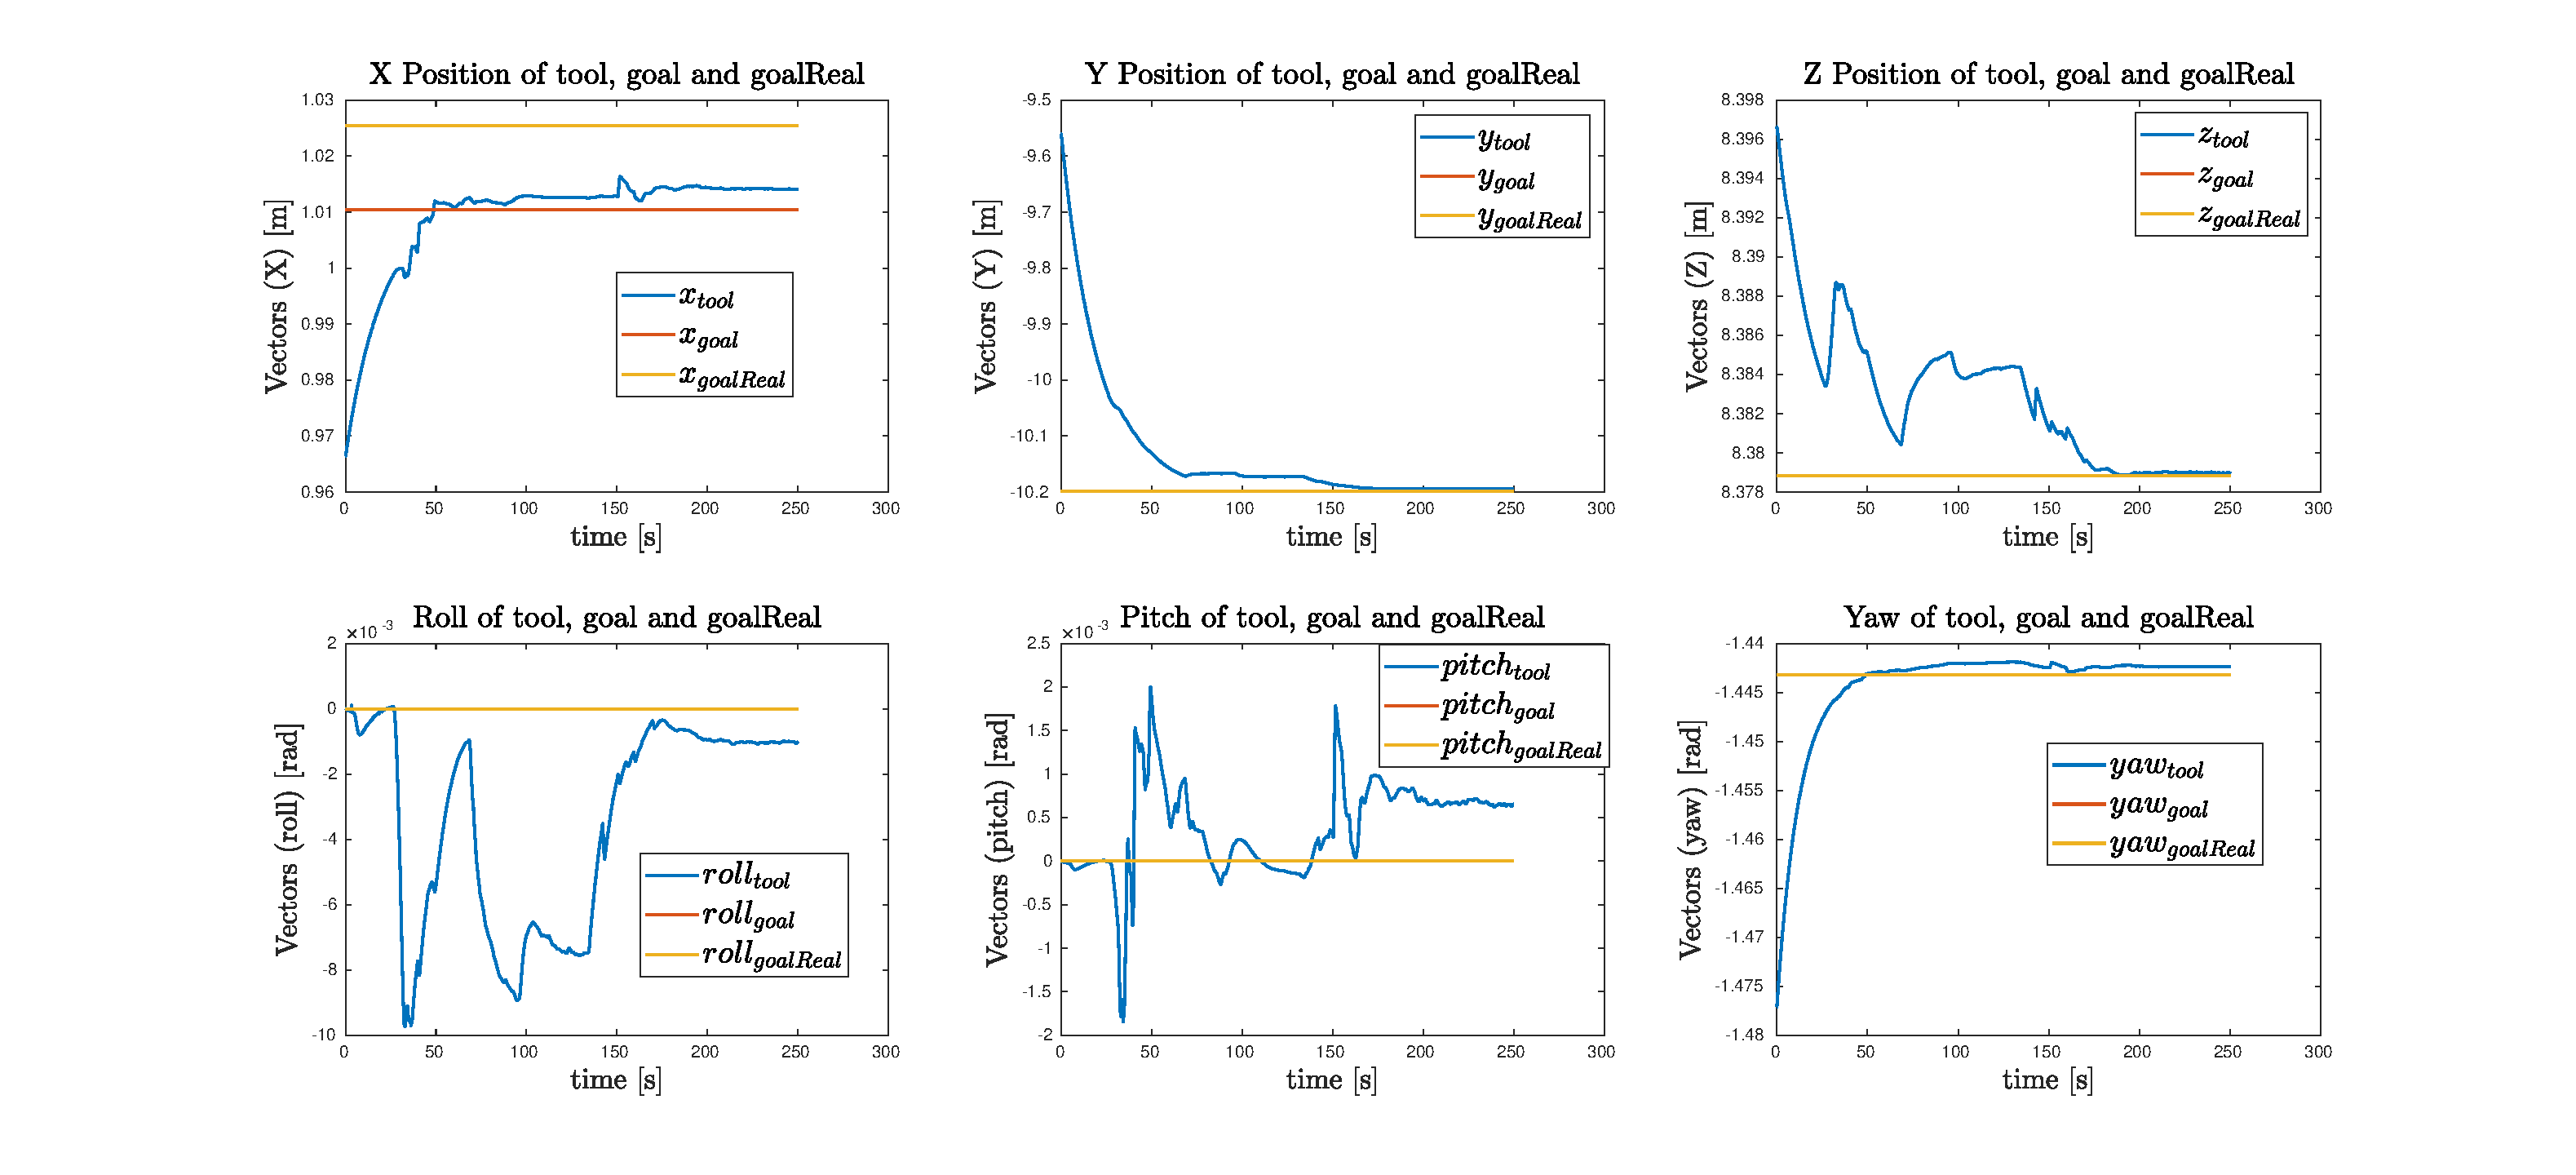
\includegraphics[width=22cm]{error_nothing/6_error.eps}
	}
	\vspace{15px}
\textbf{With Change Goal routine}
	\centerline{
		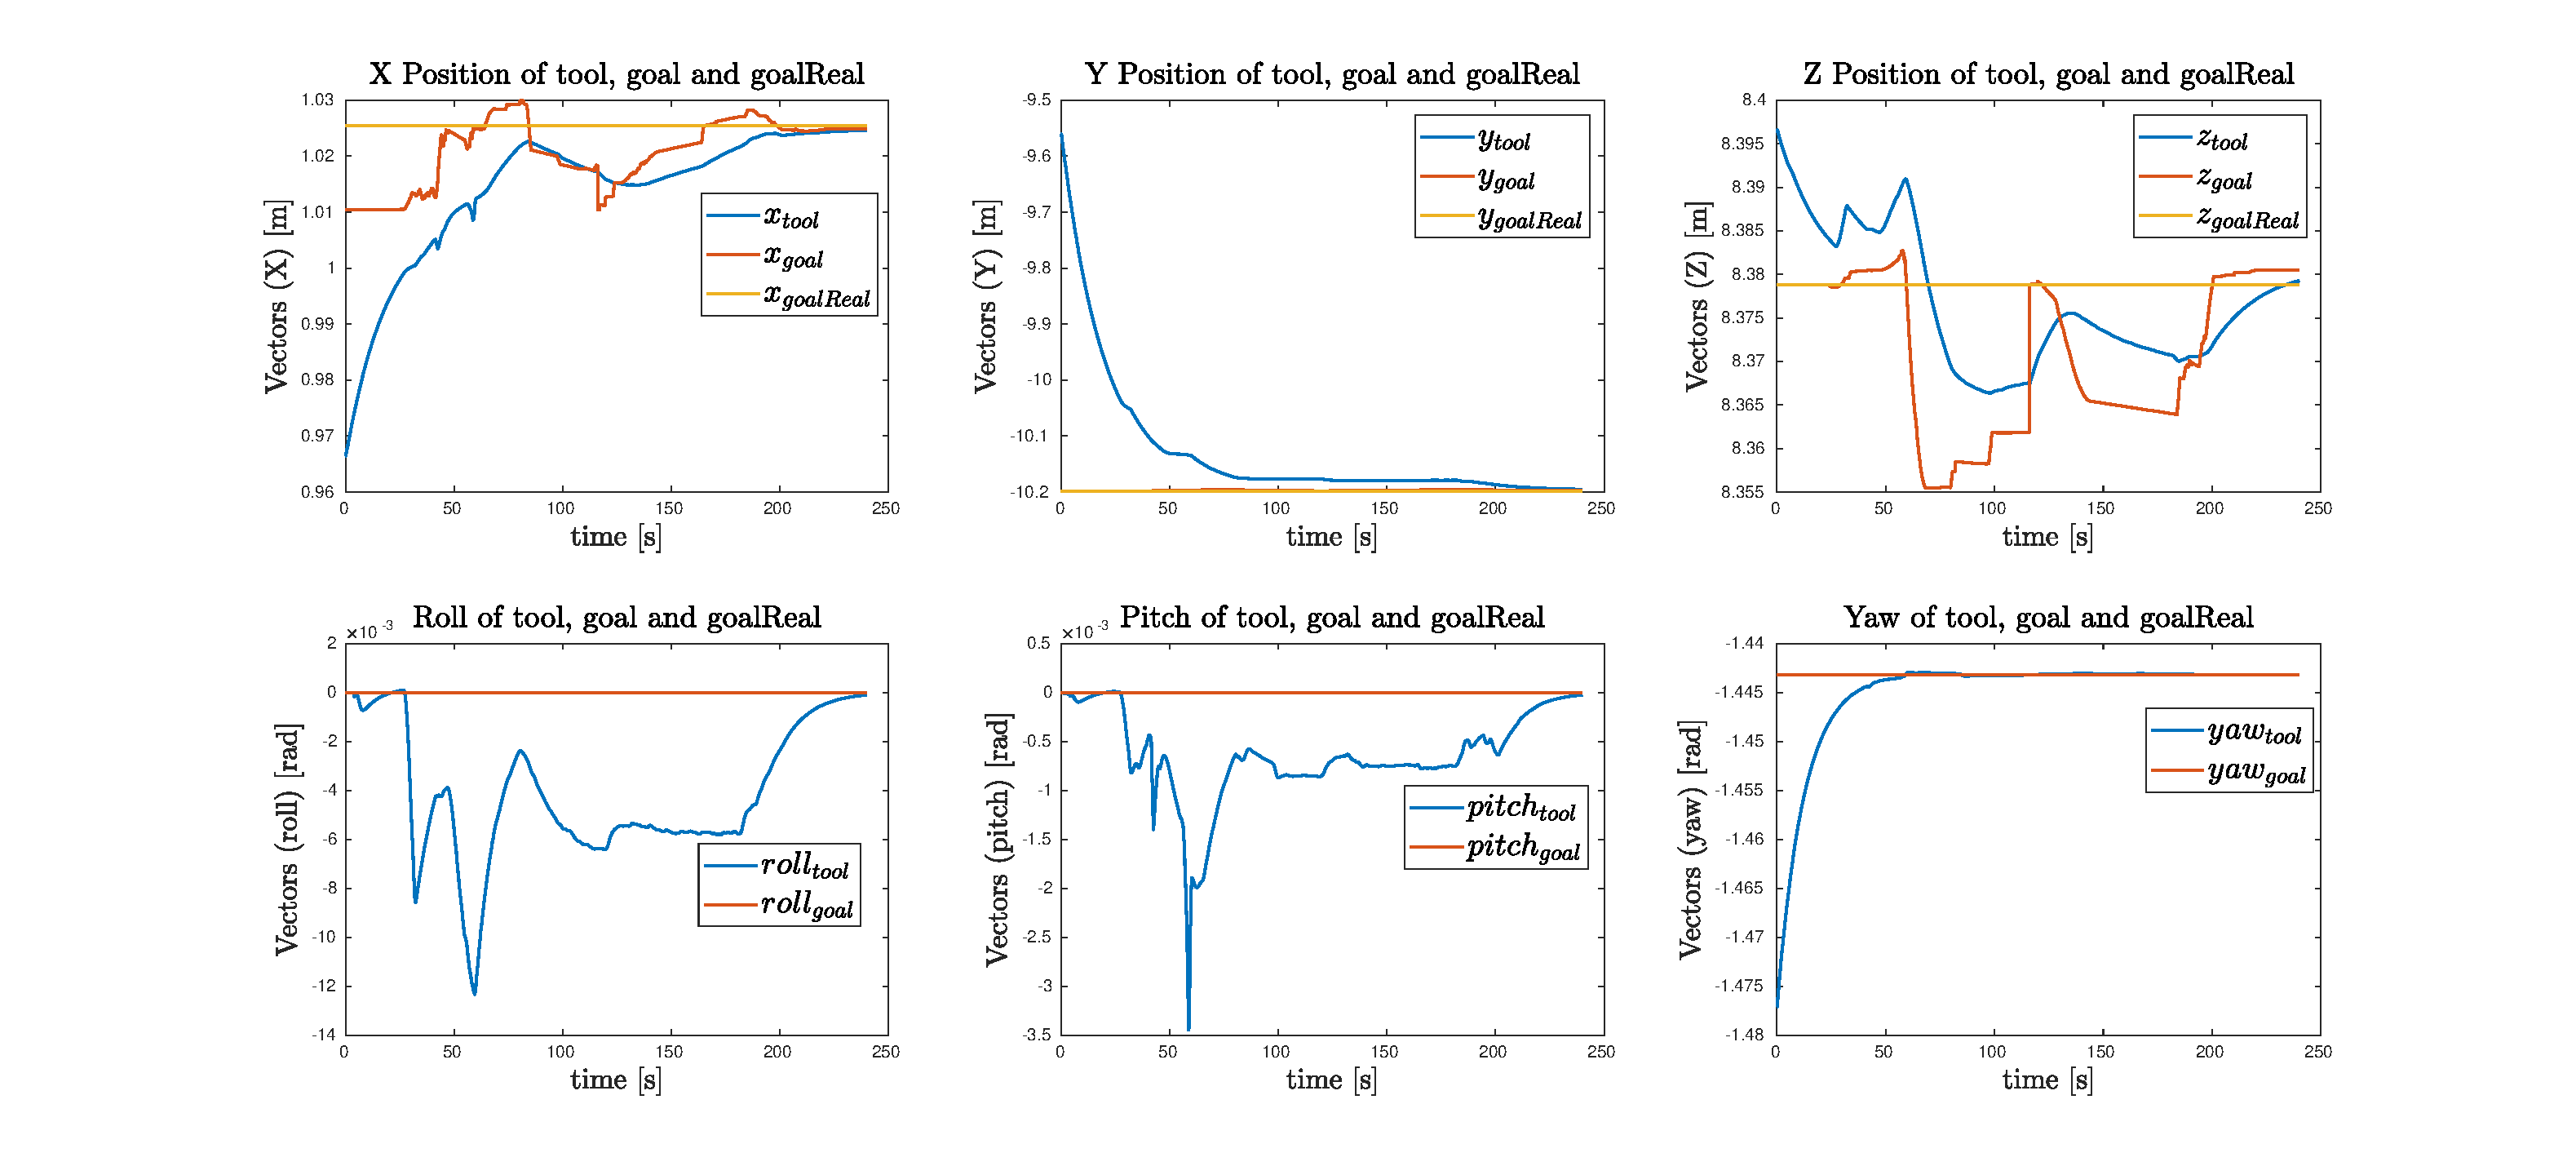
\includegraphics[width=22cm]{error_goal/6_error.eps}
	}
\end{figure} 
\captionof{figure}[Plots of Tool and Goal frames with and without changing the goal]{Results of the two experiment without and with the Change Goal routine (both without the Force-Torque objective). The plots show the pose of the goal frame $ \langle t \rangle$ and of the tool's tip frame divided into their linear and angular components. The upper six plots show results without the routine which changes the goal position, the bottom ones show results with the routine. All the component are respect to the world frame. For the linear part, the yellow lines represent the position of the goal without errors. The red lines represent the position of the goal that the controller uses. Please note that in some plots the red and yellow lines are coincident because the component is know without errors \emph{and} it is not modified. It is clearly visible that, when the goal is modified, the red line goes toward the yellow one, \textit{correcting} the initial hole's pose error.}
\label{fig:Error_nothingandgoal_plot6}
\vspace{40px}




\begin{figure}[H]
	\centering
	\textbf{Error of 0.015 meter on x-axis of the goal\\}
	\vspace{30px}
	\textbf{Norm of the forces and torques acting on the peg\\}
	\vspace{10px}
	\centerline{
	\hspace{5px}
	\textbf{Without Change Goal routine} 
	\hspace{35px}
	\textbf{With Change Goal routine}
	\hspace{25px}
	\textbf{With Change Goal and Force Task} 
	}
	\centerline{ 
		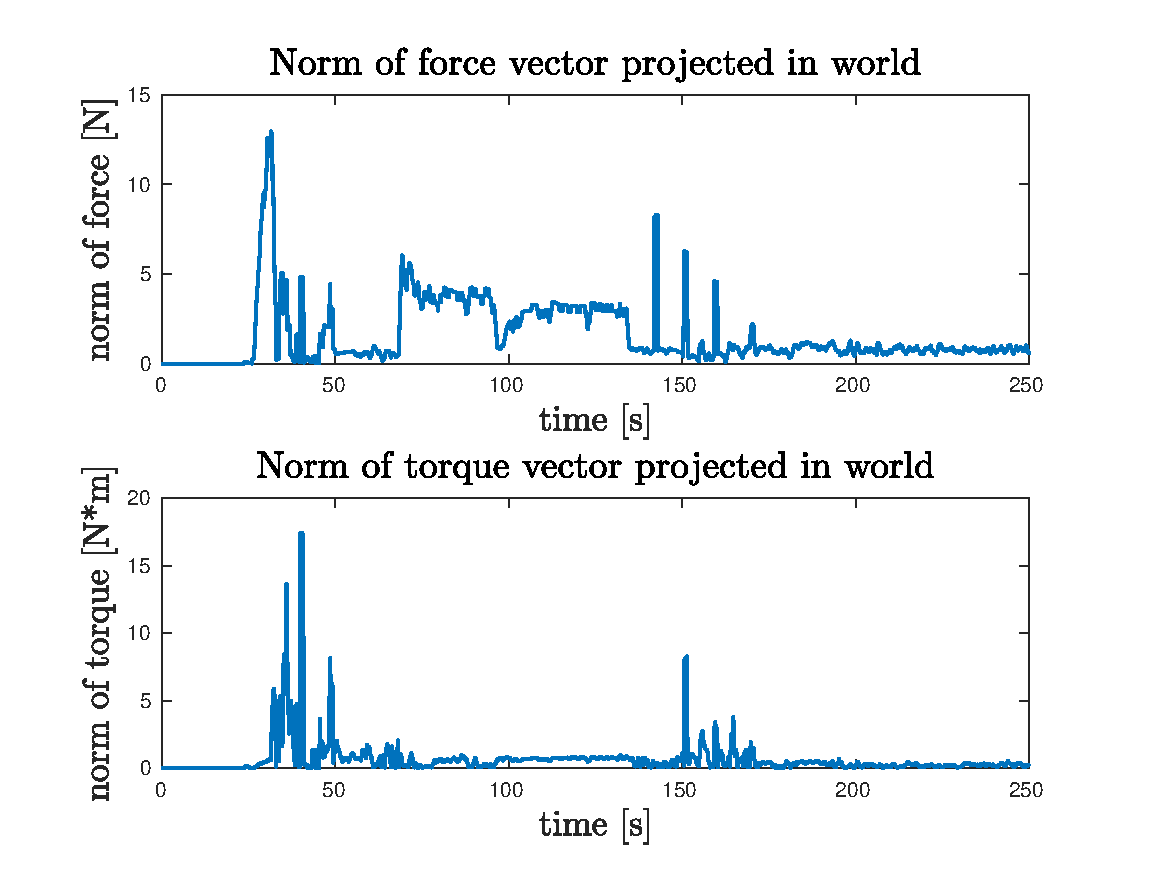
\includegraphics[width=6.5cm]{error_nothing/forcesNorm.eps}
		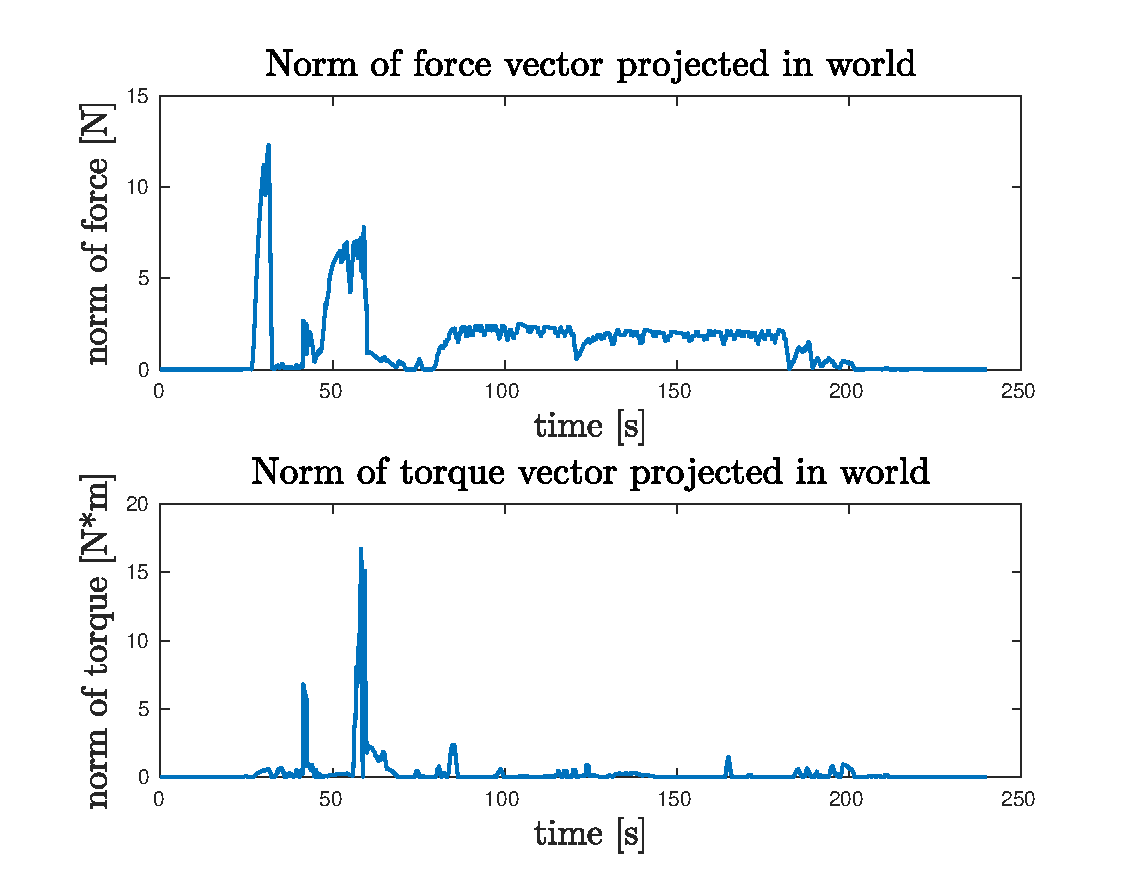
\includegraphics[width=6.5cm]{error_goal/forceNorm.eps}
	 	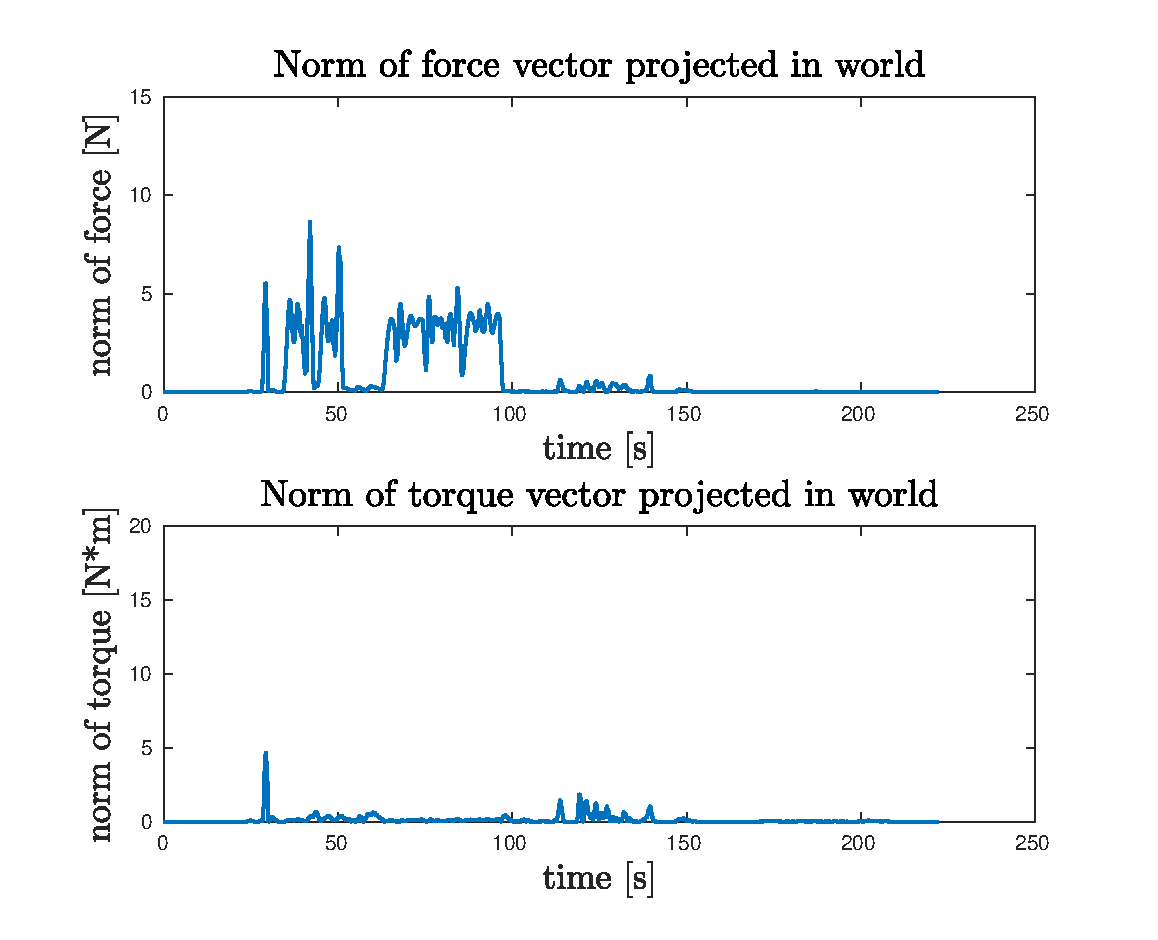
\includegraphics[width=6.5cm]{error_all/forceNorm.eps}
	}
	\vspace{30px}
	\textbf{Norm of the error between ideal goal (without the added error) and tool's tip\\}
	\vspace{10px}
	\centerline{
		\hspace{5px}
		\textbf{Without Change Goal routine} 
		\hspace{35px}
		\textbf{With Change Goal routine}
		\hspace{25px}
		\textbf{With Change Goal and Force Task} 
	}
	\centerline{
		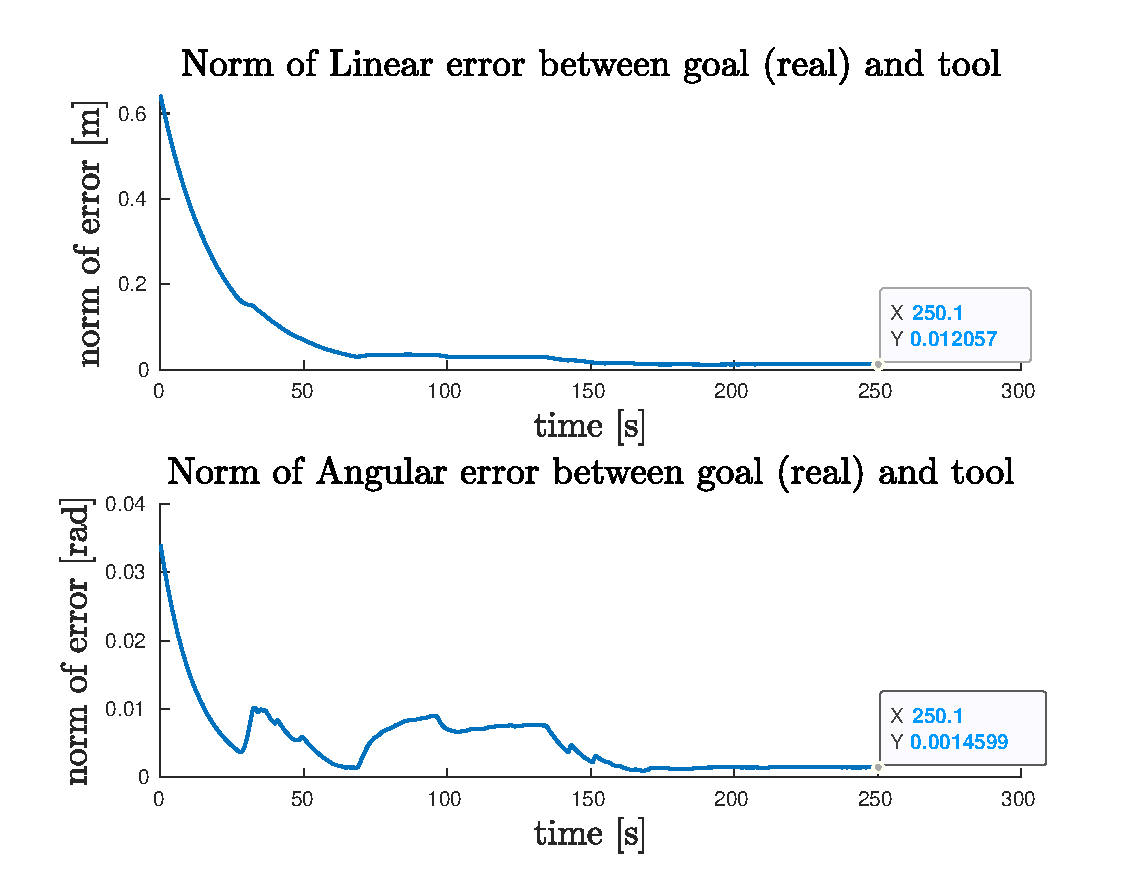
\includegraphics[width=6.5cm]{error_nothing/error.eps}
		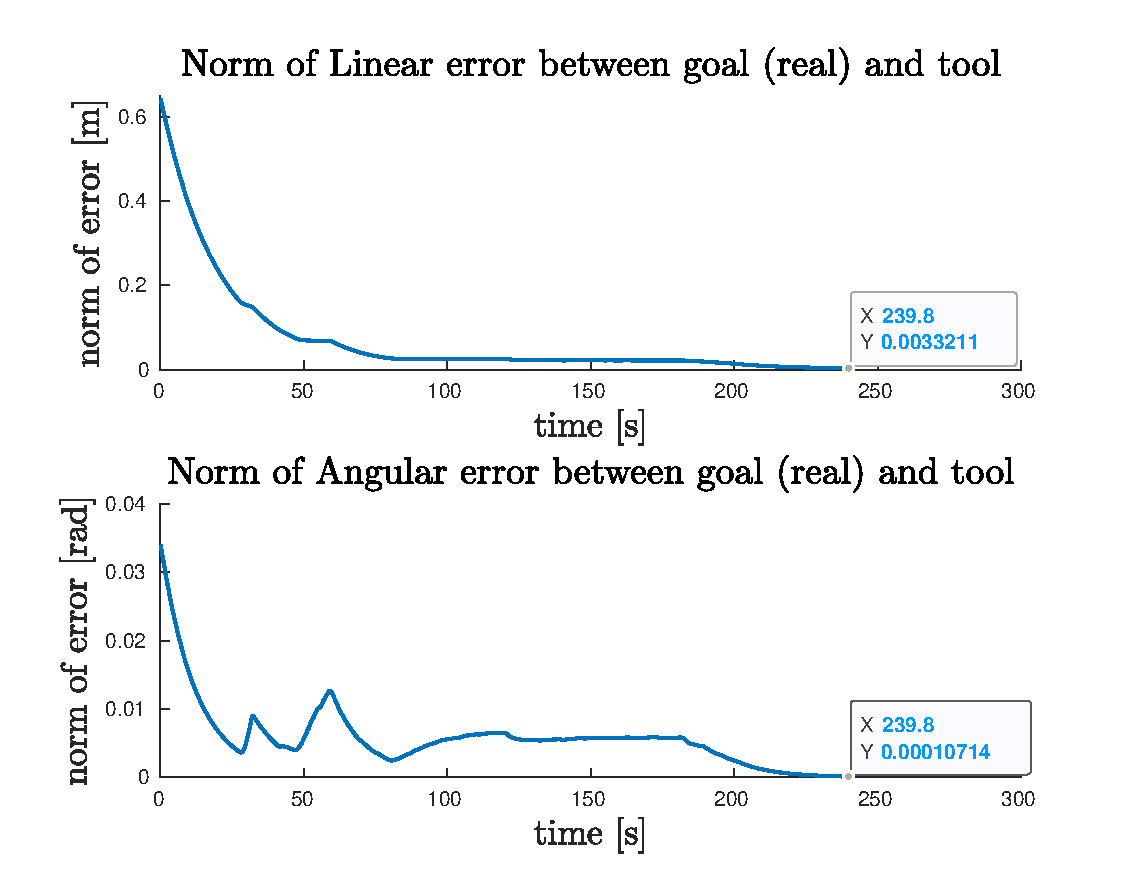
\includegraphics[width=6.5cm]{error_goal/errorNorm.eps}
		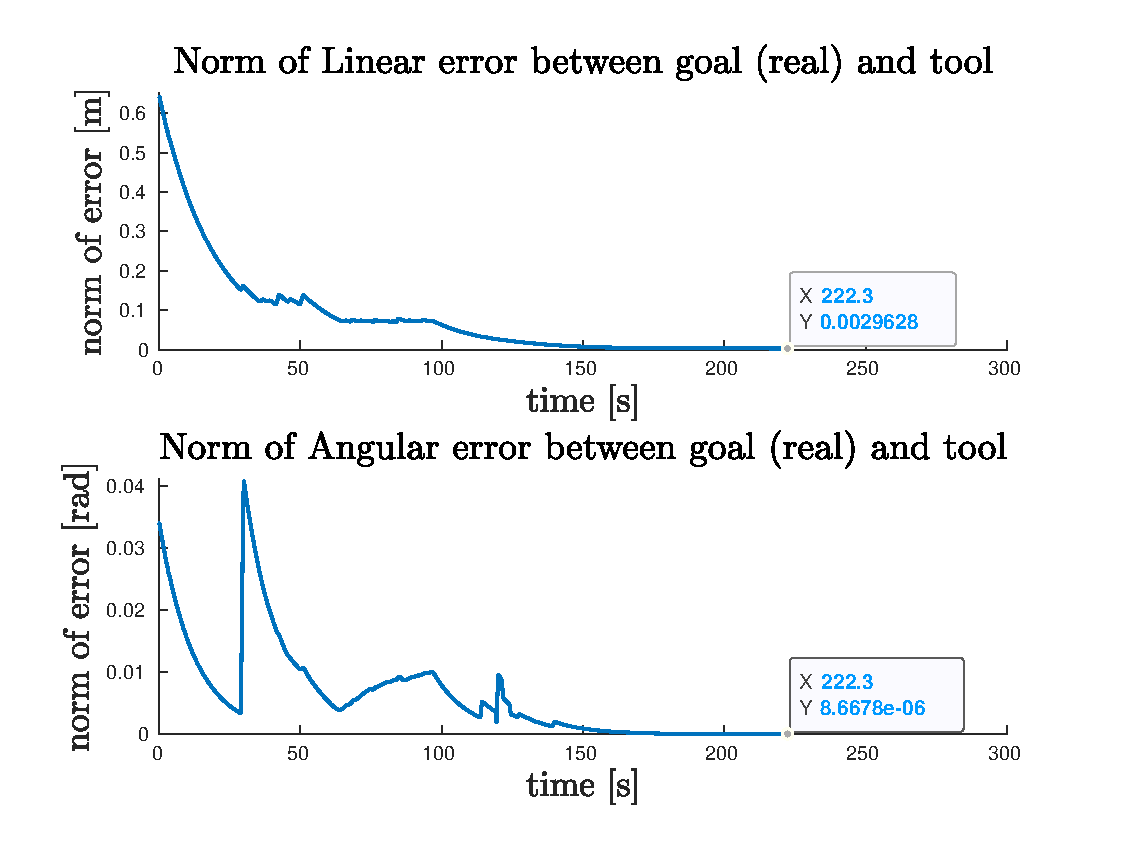
\includegraphics[width=6.5cm]{error_all/errorNorm.eps}
	}
	\vspace{10px}
	\caption[Plots of comparisons with and without change goal and force objective]{Comparison of results of the three methods: vanilla, Change Goal and Change Goal with Force-Torque objective. The three upper plots show the norm of the force and of the torque acting on the peg. It can be noticed that, in the cases where the goal is modified, at the end their norms goes to zero. The three lower plots show the norms of the error between goal and tool's tip. In the case without the Change Goal routine, the norms converge anyway but to a slightly bigger value than the one of the other two cases. In fact, when the Change Goal routine is used, the initial pose error tends to be corrected.}
	\label{fig:comparison_final}
\end{figure}

\begin{figure}[H]
	\centering
	\textbf{Error of 0.015 meter on x-axis of the goal\\}
	\textbf{with Change Goal routine and Force-Torque objective}\\
	\vspace{13px}
	\textbf{Forces and torques acting on the peg\\}
	\vspace{3px}
	\centerline{ 
		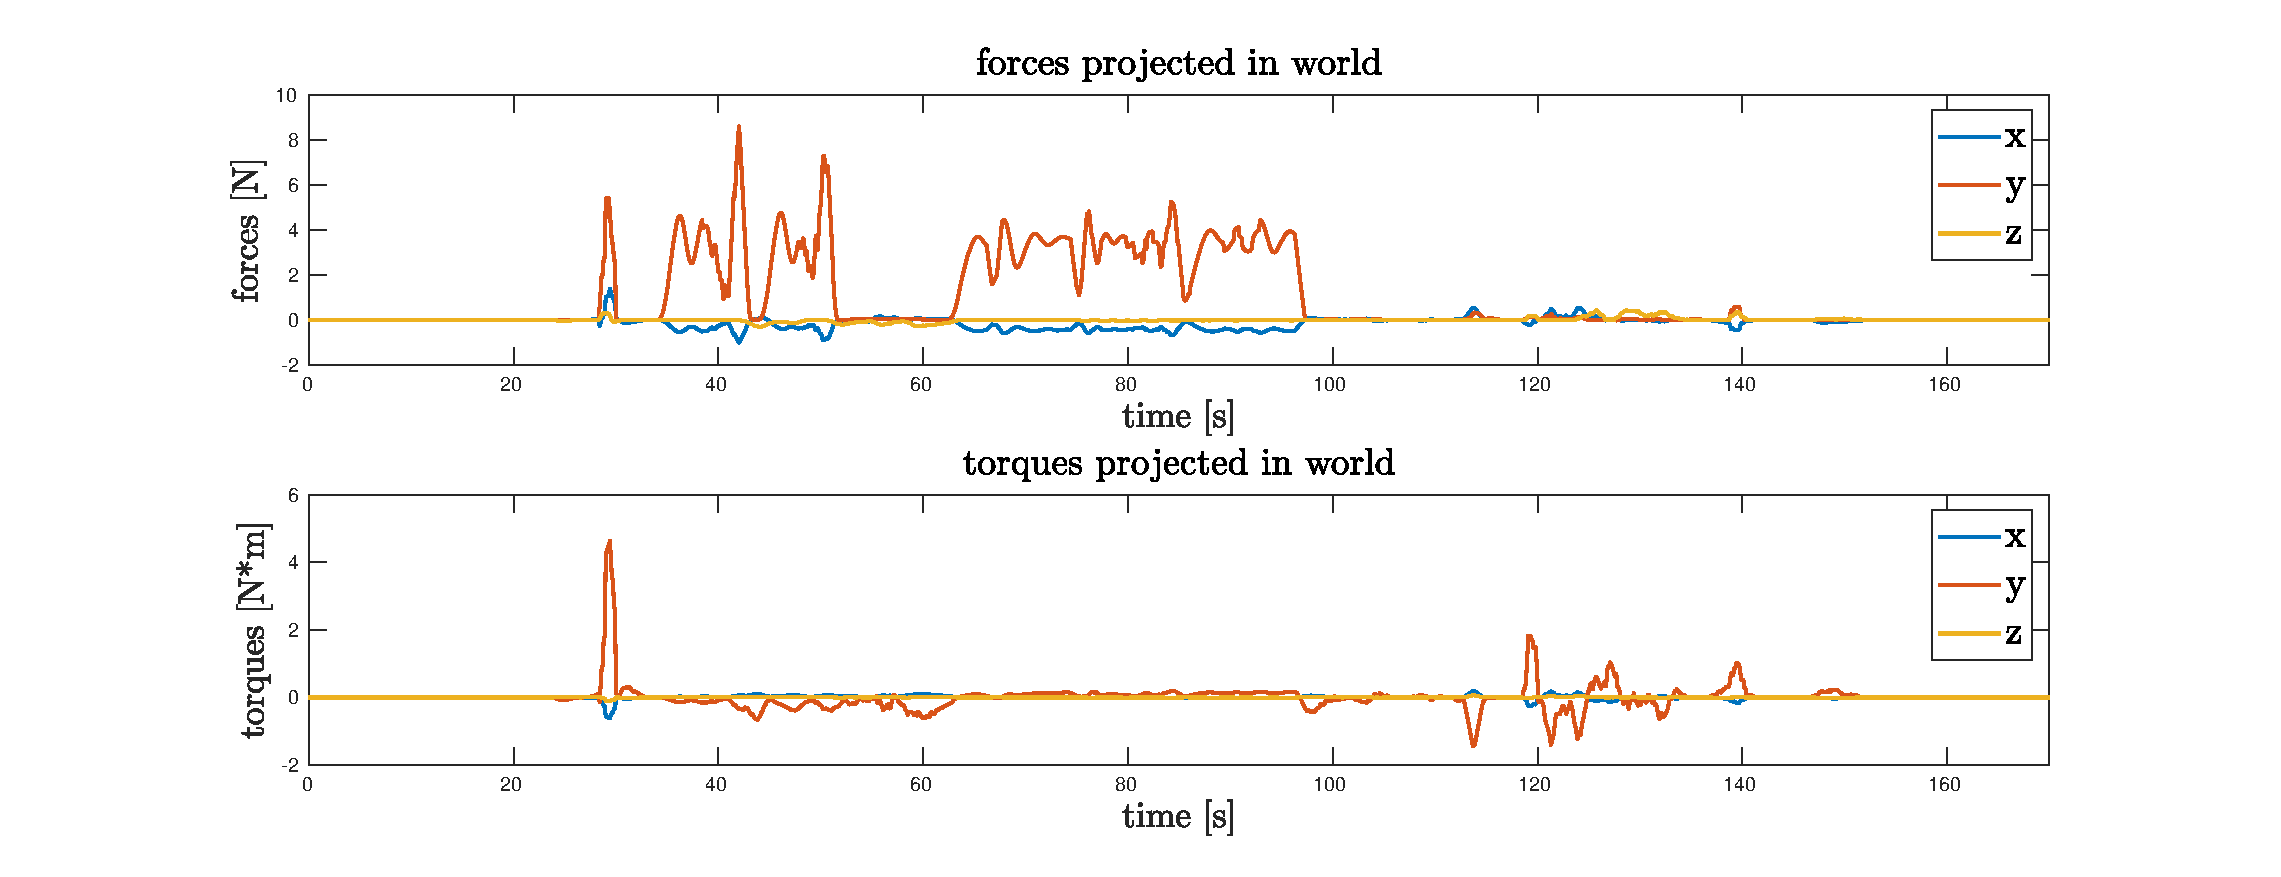
\includegraphics[width=15.5cm]{error_all/force.eps}
	}
	\vspace{10px}
	\textbf{Force-Torque objective: References and Activations\\}
	\vspace{3px}
	\centerline{
		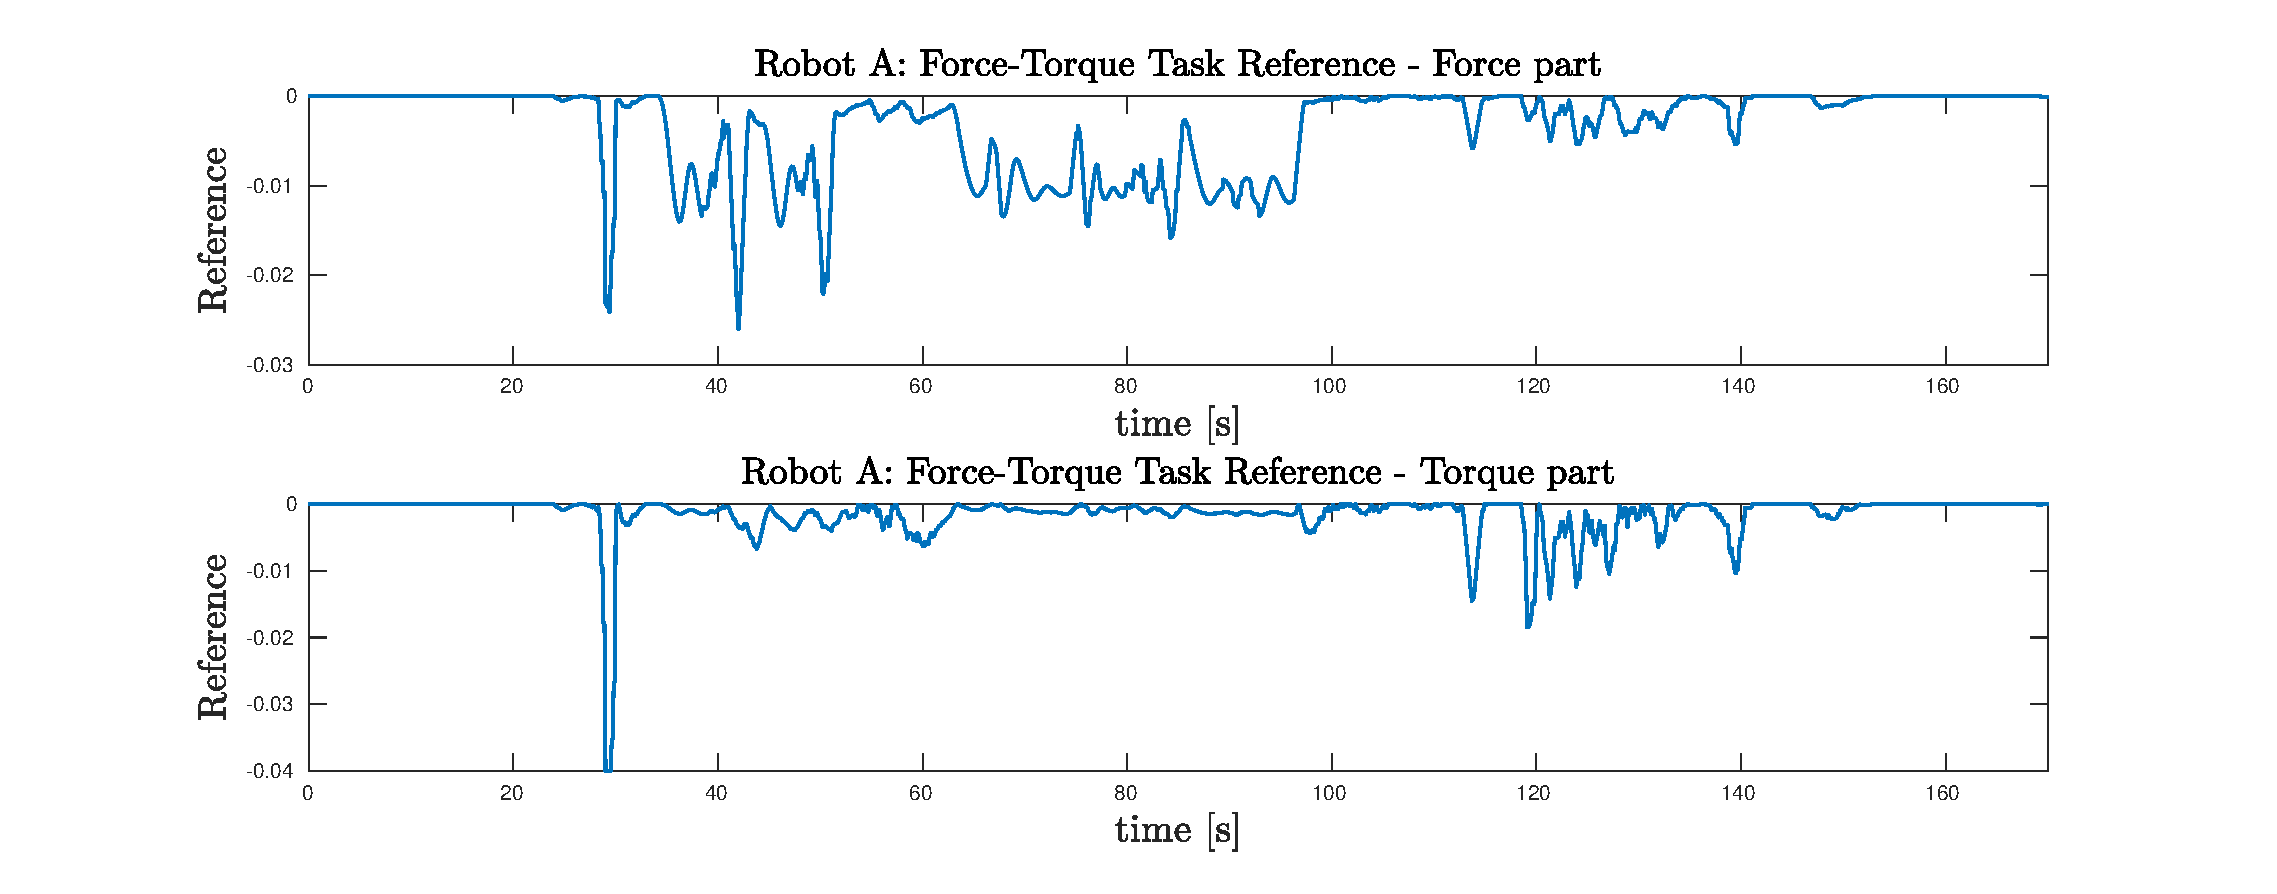
\includegraphics[width=15.5cm]{error_all/referenceForceTask.eps}
	}
	\centerline{
		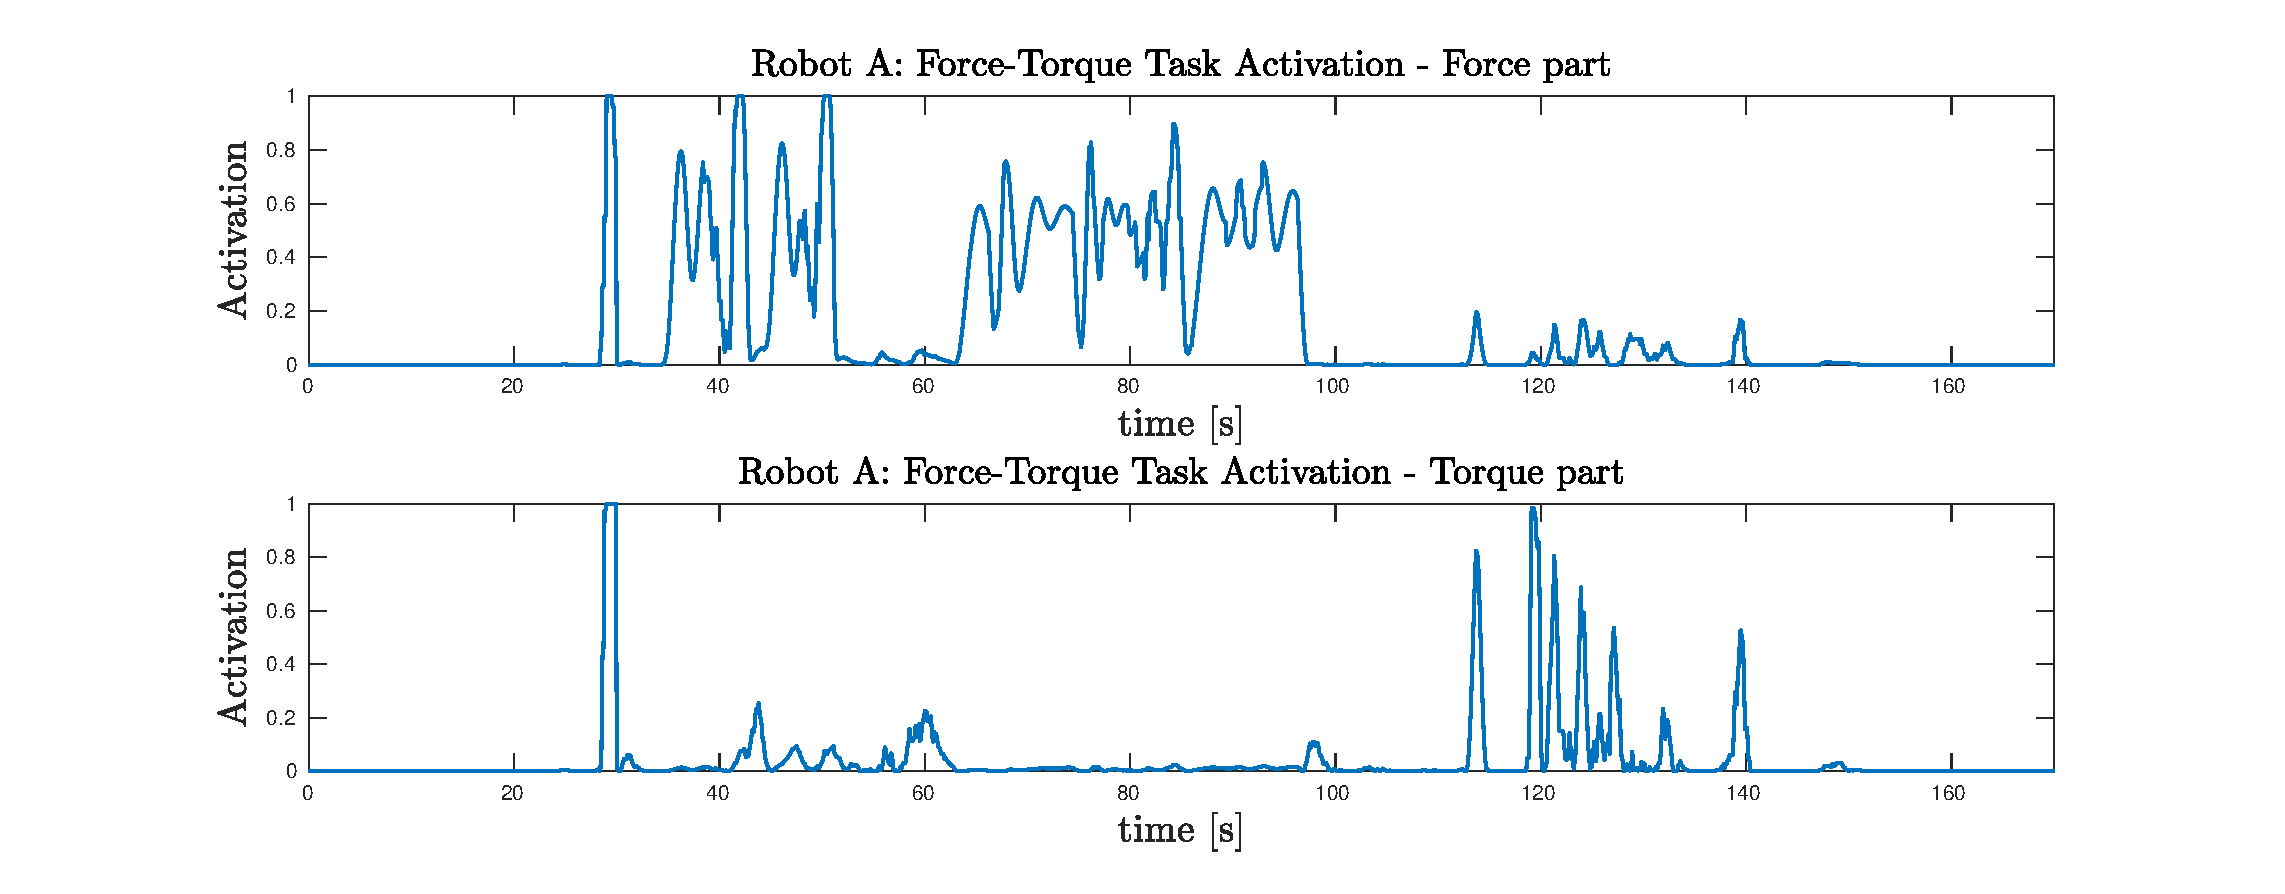
\includegraphics[width=15.5cm]{error_all/activationForceTask.eps}
	}

	\caption[Plots with reference and activation of the force task]{The forces and torques acting on the peg (above), and the corresponding generated references and activations  of the Force-Torque objective (below); they are calculated by robot A, but for robot B they are the same.}
	\label{fig:forceTaskActRef}
\end{figure}

\begin{figure}[H]
	\centering
	\textbf{Results with error of 0.015 meter on x-axis of the goal}\\
	\textbf{with Change Goal routine and Force-Torque objective}\\
	\vspace{15px}
	\textbf{Velocities generated by the Force-Torque objective only\\}
	\vspace{5px}
	\centerline{ 
		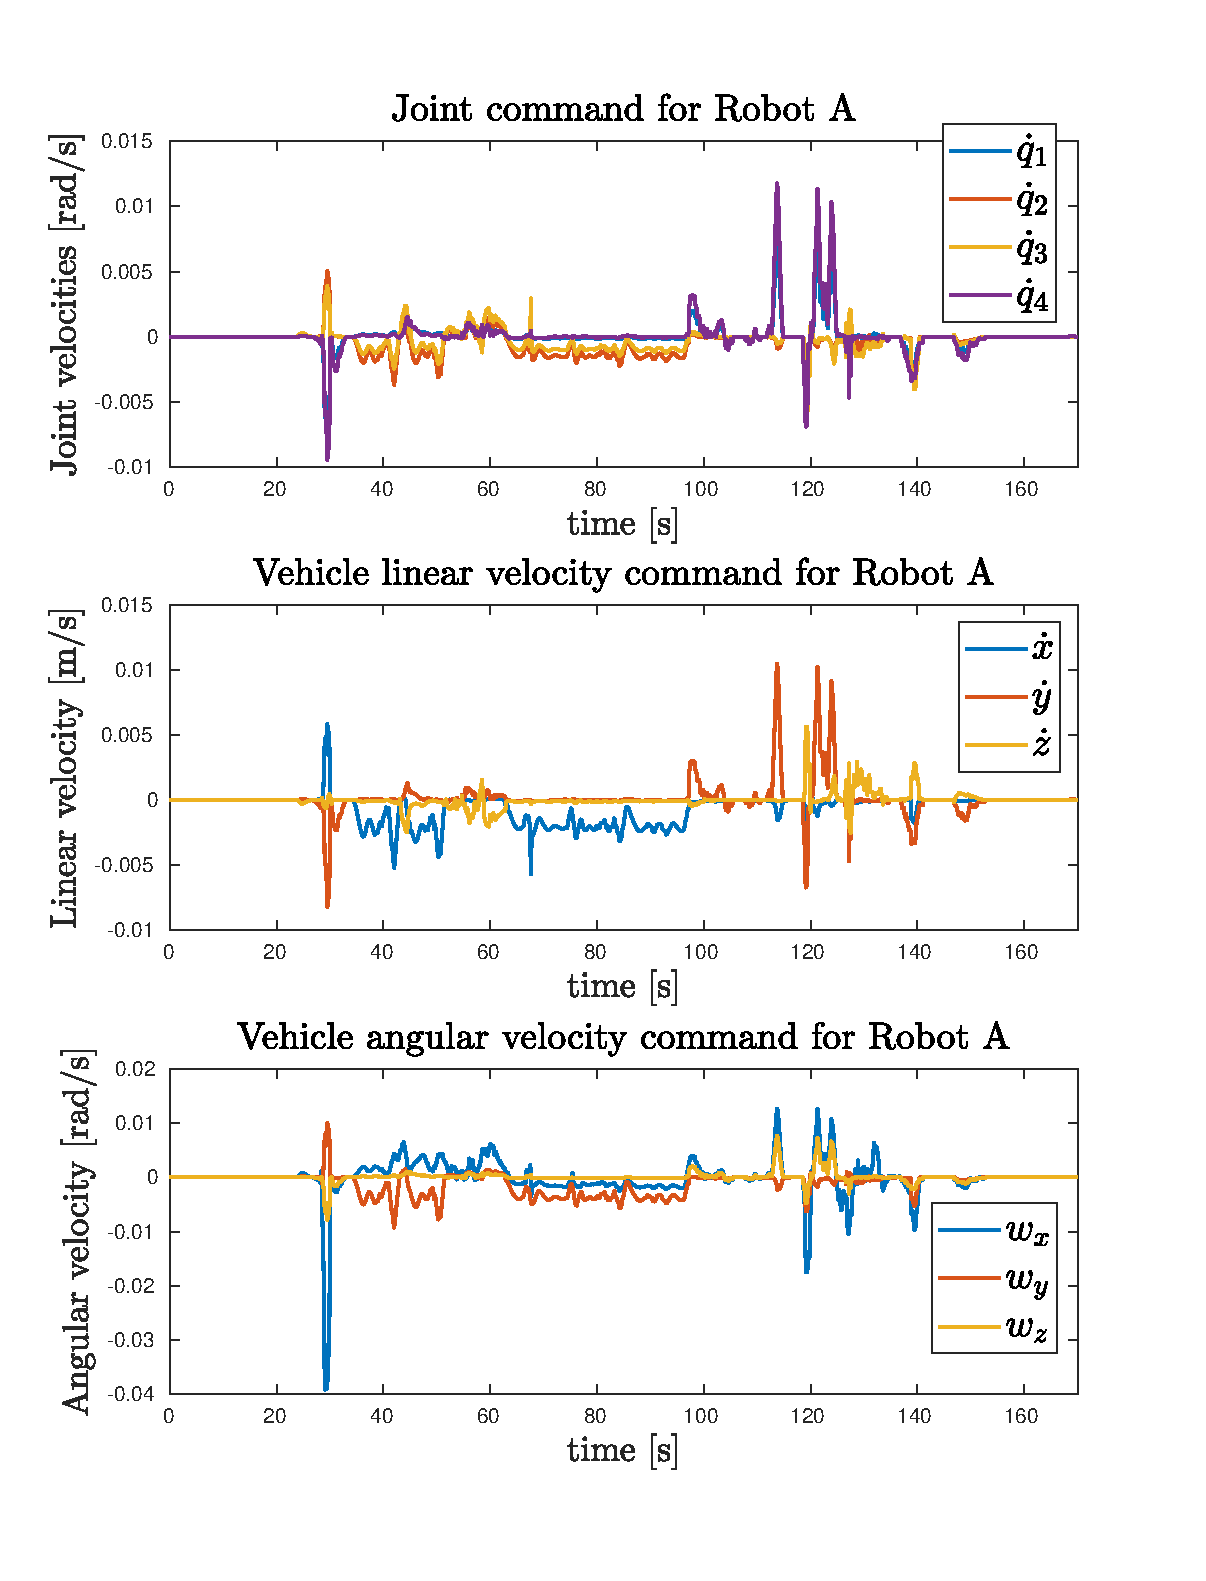
\includegraphics[width=9cm]{error_all/velocityForceTaskA.eps}
		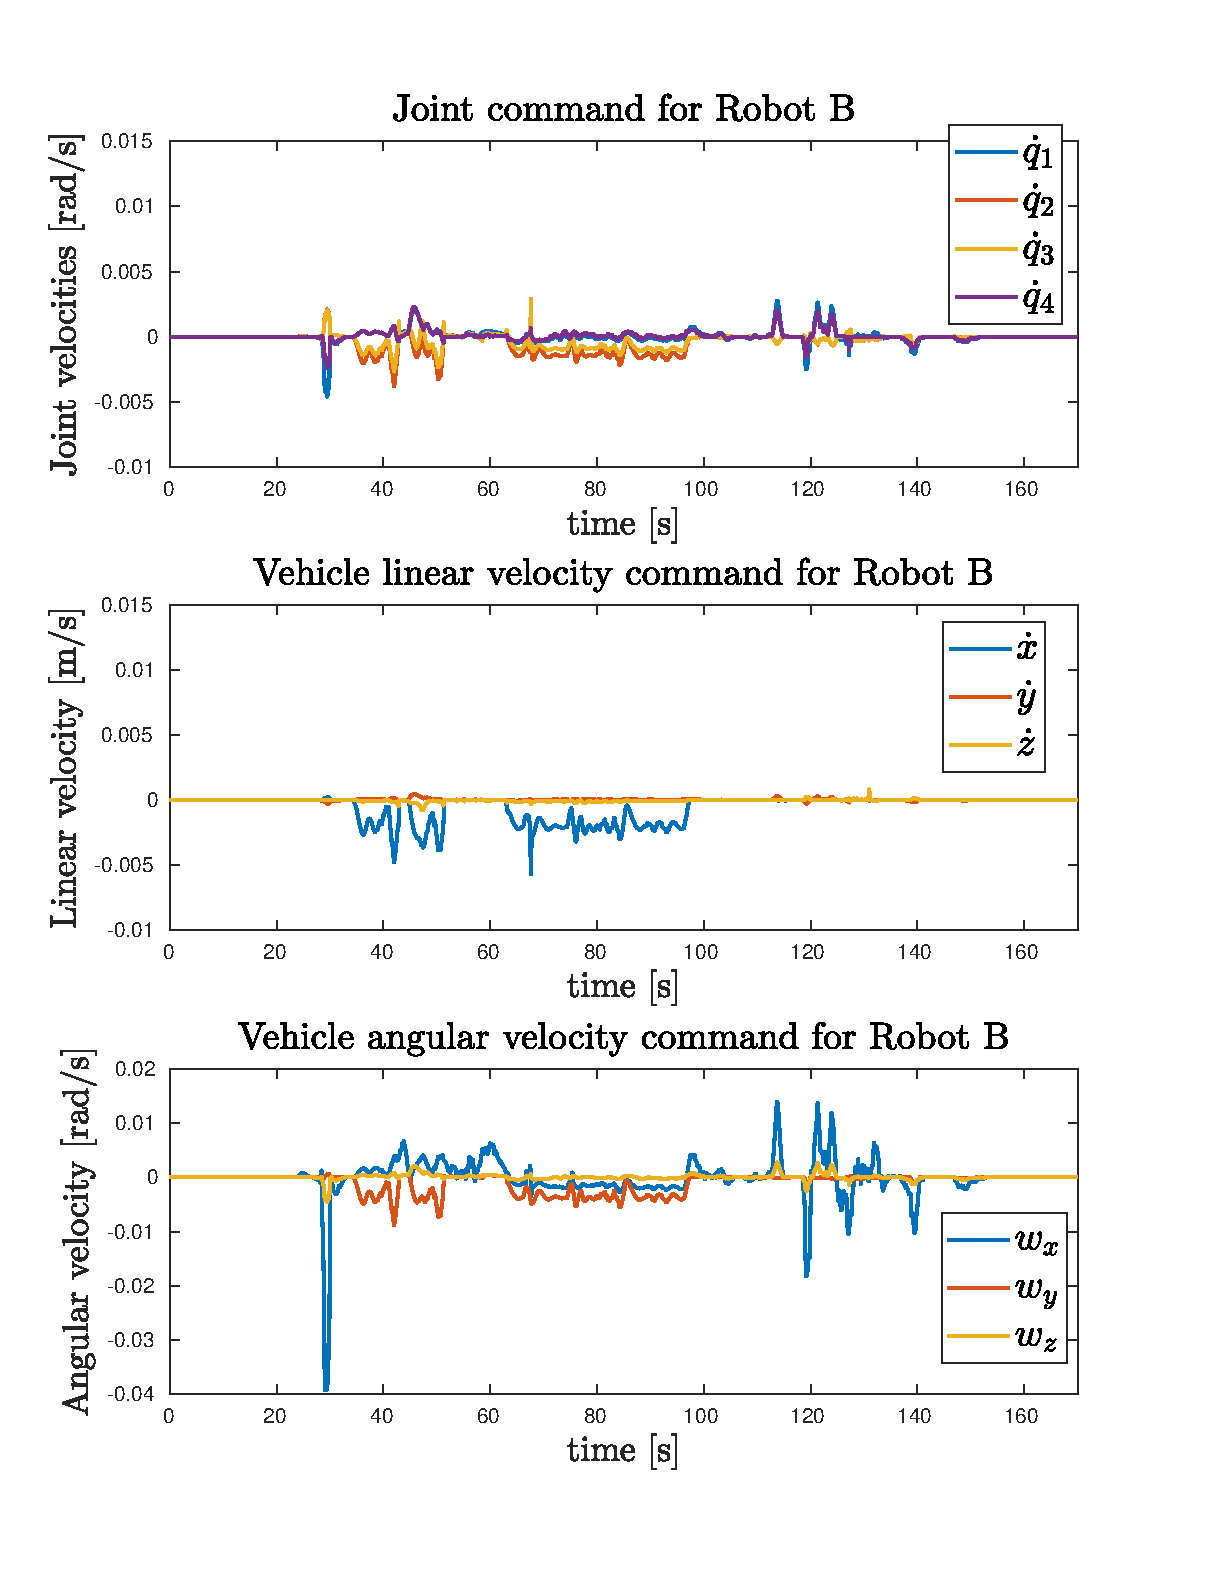
\includegraphics[width=9cm]{error_all/velocityForceTaskB.eps}
	}
	
	\caption[Plots of the velocity command generated by the Force-Torque objective]{The velocity command generated by the Force-Torque objective, for the Robot A. These are the velocities that the task generates; the vectors depicted are simply the result of $\; \boldsymbol{J}^{\#}_{ft} \; \dot{\bar{\boldsymbol{x}}}_{ft}\;$ to show how the objective works. So they are not the real one applied to the system because with this formula higher priority objectives are not taken into consideration. For the two robots, the reference $\dot{\bar{\boldsymbol{x}}}_{ft}$ is the same because they act with the same data, it is the Jacobian $\boldsymbol{J}^{\#}_{ft}$ which is obviously different and which makes the two plots dissimilar.}
	\label{fig:forceTaskVelocities}
\end{figure}


\section{Results with the Hole's pose estimation by Vision}
\label{sec:finalTest}
\begin{figure}[H]
	\centering
	\includegraphics[width=11cm, height=5.3cm]{uwsim_scenario_all0.png}
	\includegraphics[width=11cm, height=3.2cm]{uwsim_scenario_all1.png}
	
	\caption[Scenatio for the final test with Vision]{The starting position of the robots for the final experiment, where it is used the preliminary phase to estimate the hole's pose with vision.}
	\label{fig:uwsim_expAll}
\end{figure}
Here, results with the preliminary vision phase are shown. Differently from the previous experiments of section \ref{subsec:resultsControlError}, the error of the hole's pose when using the Vision Robot is not so influential on the mission. In norm, the pose estimation error is less than $0.006$ meters for the linear part and $0.01$ radians for the angular part (with the best method, as shown in figure \ref{fig:squareErrors} of section \ref{subsec:trackResult}).\\ 
However, the experiment is interesting not only because it puts all the mission phases together, but also because it shows the outcome when the error is \enquote{spread} among all linear and, especially, angular component (which was not considered before). Even more, the carrying robots start farther from the hole than before. In this simulation, both the Change Goal routine and the Force-Torque objective are used.\\
The test's details described at the beginning of section \ref{sec:resultNoVisio} are still valid, except for the initial position of the two carrying robot. This time, the distance between hole and peg's tip has component $[3.590, 0.039, -0.041]$ for the linear part (and the same as previous for the angular part: $[0, 0, 1.942]$ \textit{roll, pitch, yaw}, in degrees).\\
Some screenshots that show the main phases of the simulation are visible in figure \ref{fig:screenSimulation}. The interesting plots about the performances are shown in figure \ref{fig:expWithVisio}. To give an idea of the magnitude of the velocities involved, cooperative system velocities $\dot{\hat{\boldsymbol{y}}}_a$ and $\dot{\hat{\boldsymbol{y}}}_b\,$, and cooperative tool velocity $\dot{\tilde{\boldsymbol{x}}}_t$ are displayed in figure \ref{fig:expWithVisioVel} and figure \ref{fig:expWithVisioVelTool}. Please note that these velocities do not include the collision propagation and the firm grasp constraint, they are only the output of the kinematic layer.


\begin{figure}[H]
	\centering
	\textbf{Screenshots from the final experiment }\\
	\vspace{5px}
	\centerline{
		\includegraphics[width=6cm, height=3.5cm]{screenUWSIM/1new.png}
		\includegraphics[width=6cm, height=3.5cm]{screenUWSIM/2New.png}
	}
	\vspace{1px}
	\centerline{
		\includegraphics[width=6cm, height=3.5cm]{screenUWSIM/3.png}
		\includegraphics[width=6cm, height=3.5cm]{screenUWSIM/4.png}
	}
		\vspace{1px}
	\centerline{
		\includegraphics[width=6cm,height=3.5cm]{screenUWSIM/5.png}
		\includegraphics[width=6cm, height=3.5cm]{screenUWSIM/6.png}
	}
		\vspace{1px}
	\centerline{
		\includegraphics[width=6cm, height=3.5cm]{screenUWSIM/7.png}
		\includegraphics[width=6cm, height=3.5cm]{screenUWSIM/8.png}
	}
	\caption[Screenshots from the final experiment]{Screenshots from the final experiment with Vision. From the top to the bottom, from the left to the right: a) The Vision robot has detected the squares and it is tracking the hole's pose; b) The Vision robot is driven away and the carrying robots are ready to begin; c,d) the two robots are cooperatively transporting the peg to the hole; e) The first \enquote{contact} between the \textit{peg} and the \textit{hole}; f) The \textit{peg} is being inserted; g) The robots stop because the tool has reached the desired depth (0.2m); h) A polygon wire-frame view mode of the simulator to see the \textit{peg} inserted.}

	\label{fig:screenSimulation}
\end{figure}


\begin{figure}[H]
	\centering
	\textbf{Results with hole's pose estimation by Vision}\\
	\vspace*{20px}
	\centerline{
		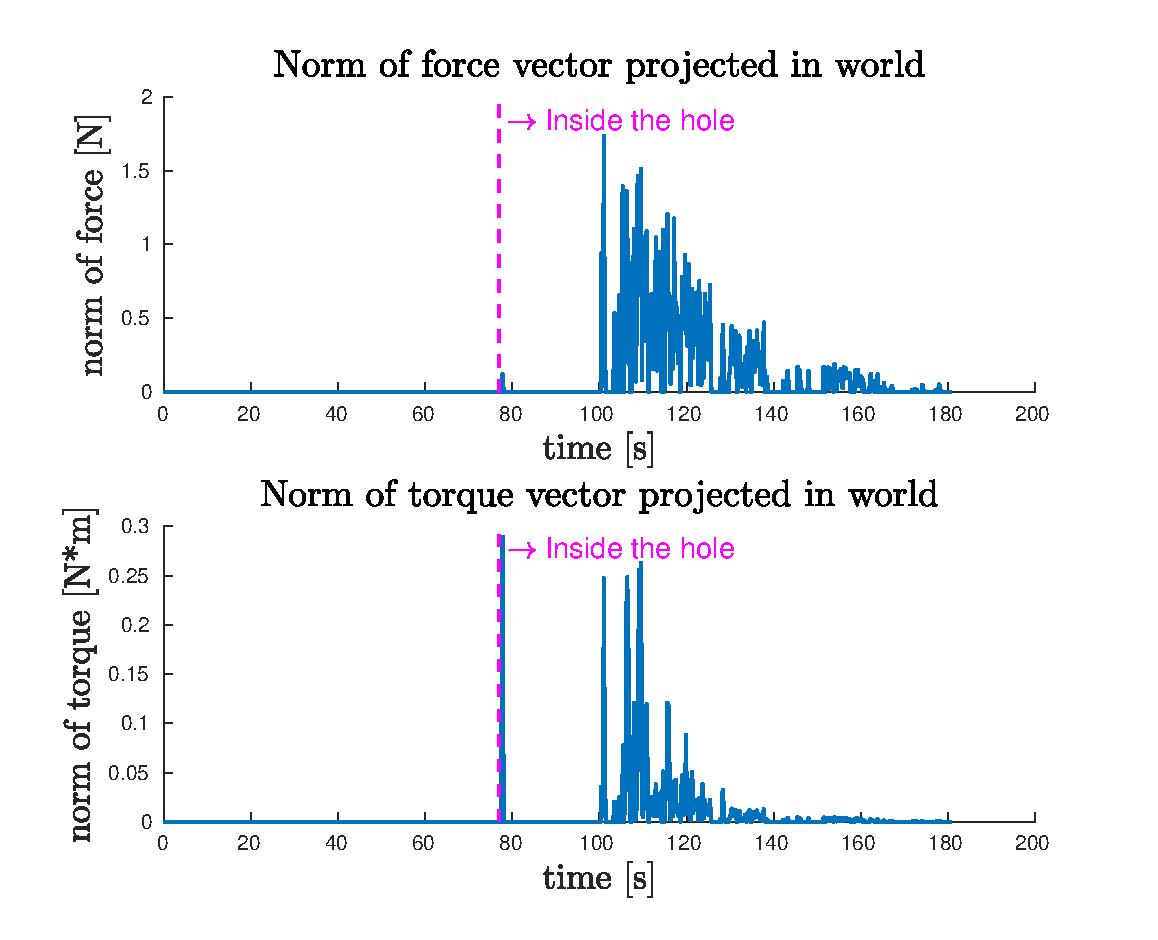
\includegraphics[width=8.5cm]{withVisio/forceNorm.eps}
		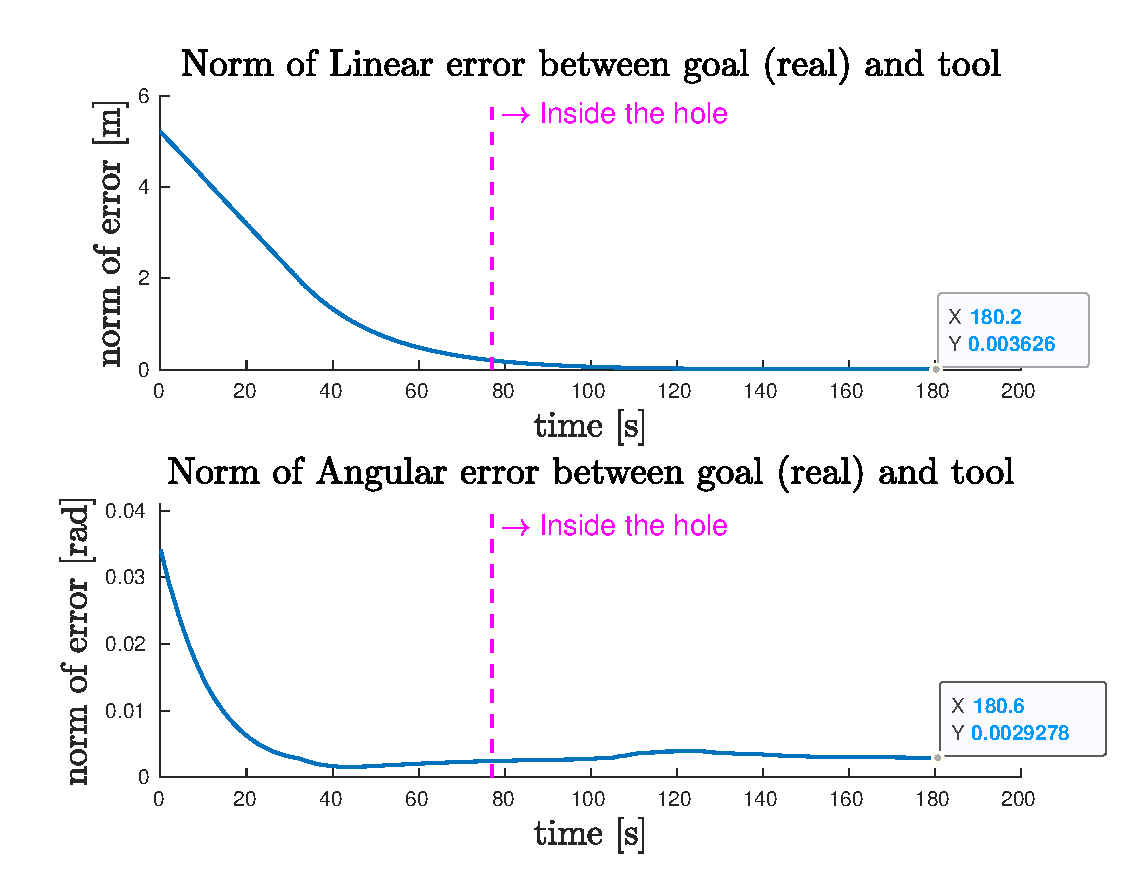
\includegraphics[width=8.5cm]{withVisio/errorNorm.eps}
	}
	\vspace{30px}
	\centerline{
		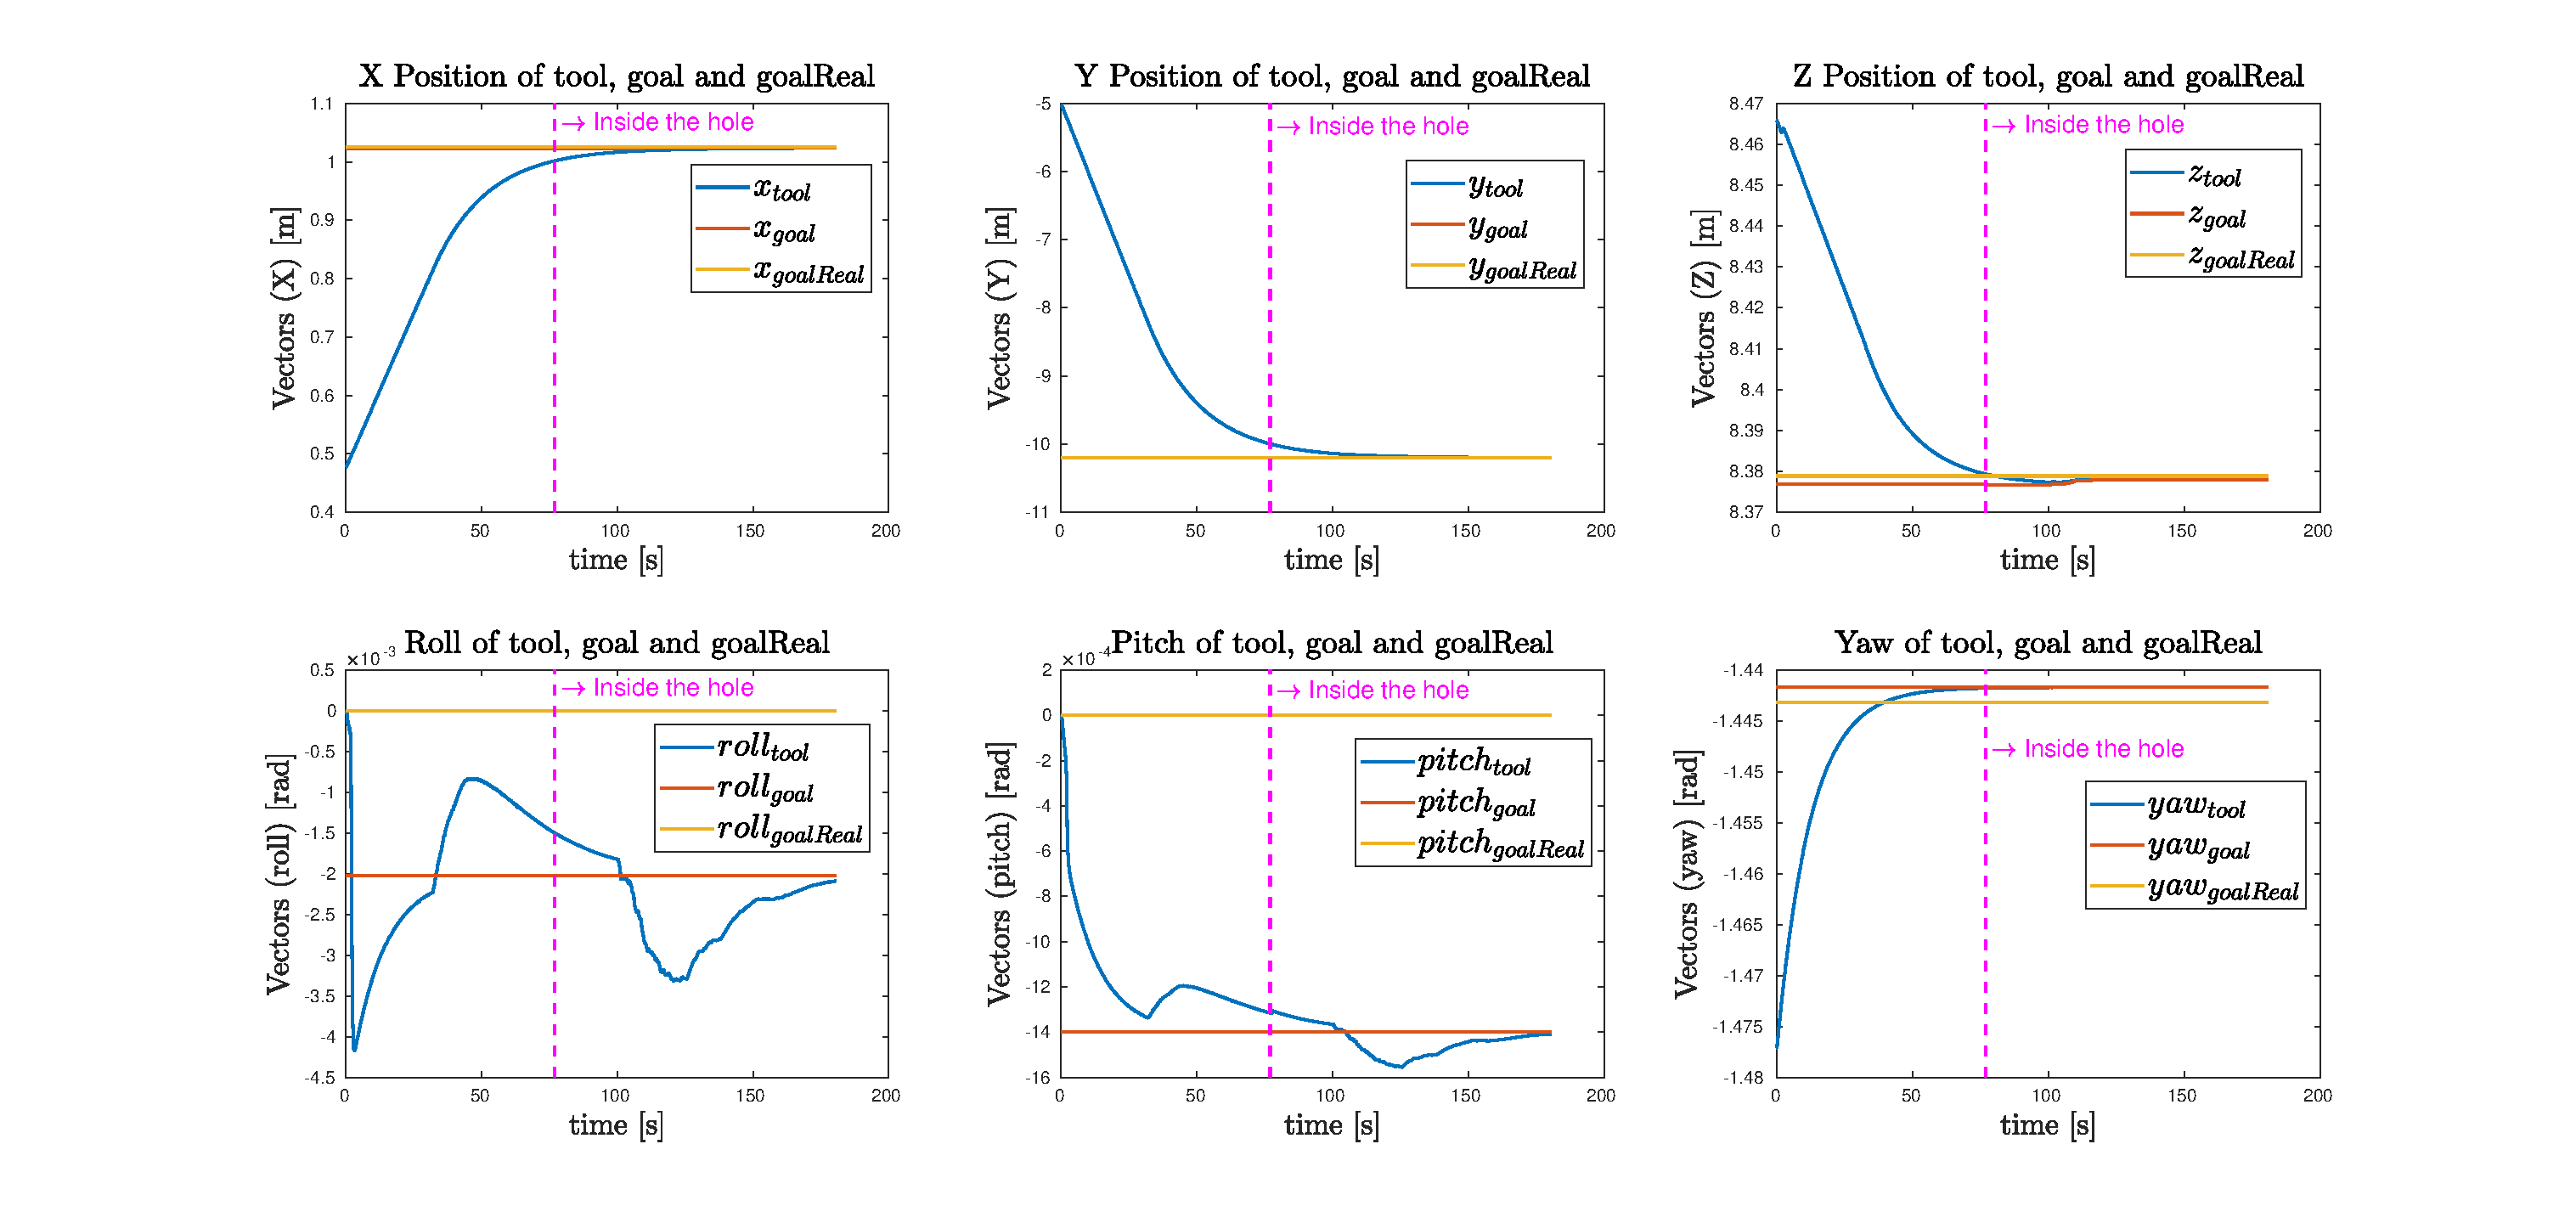
\includegraphics[width=19.5cm]{withVisio/6_error.eps}
	}
	\vspace{10px}
	\caption[Plots of results with hole's pose estimation by Vision]{Results with the hole's pose estimated by the best one of the tested vision algorithms. At second 77 the peg's tip goes inside the hole (magenta vertical lines). Being the pose estimation really good, forces and torques are not so big  as in the previous test (upper left plot). Furthermore, modification of the goal are almost not noticeable (lower plot). The positional error from goal to peg's tip  converges to a small value (upper right plot). The visible error for the angular part is due to the fact that the orientation of the goal frame has some imprecisions, due to not perfect hole's pose estimation.}
	\label{fig:expWithVisio}
\end{figure}

\begin{figure}[H]
	\centering
	\textbf{Results with hole's pose estimation by Vision}\\
	\textbf{Cooperative system velocities for robots A and B (after cooperation)}
	\vspace{20px}
	\centerline{
		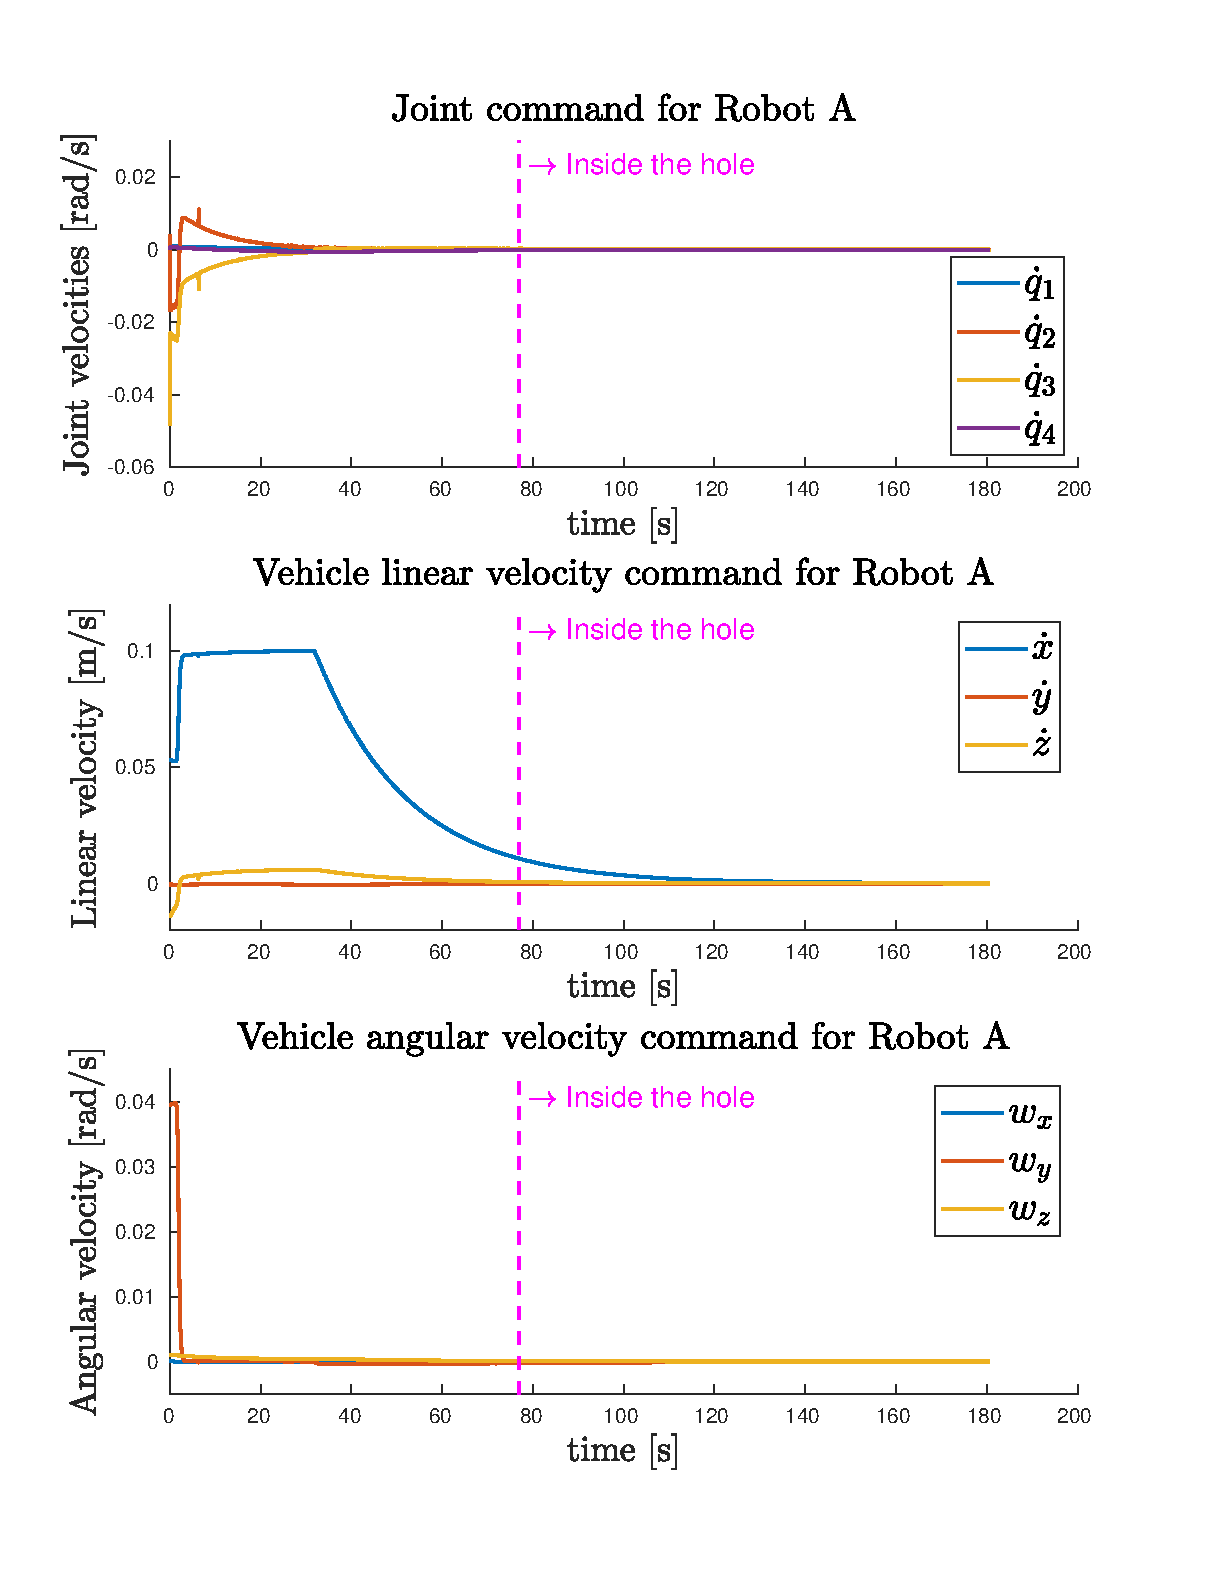
\includegraphics[width=9cm]{withVisio/coopJoinVelA.eps}
		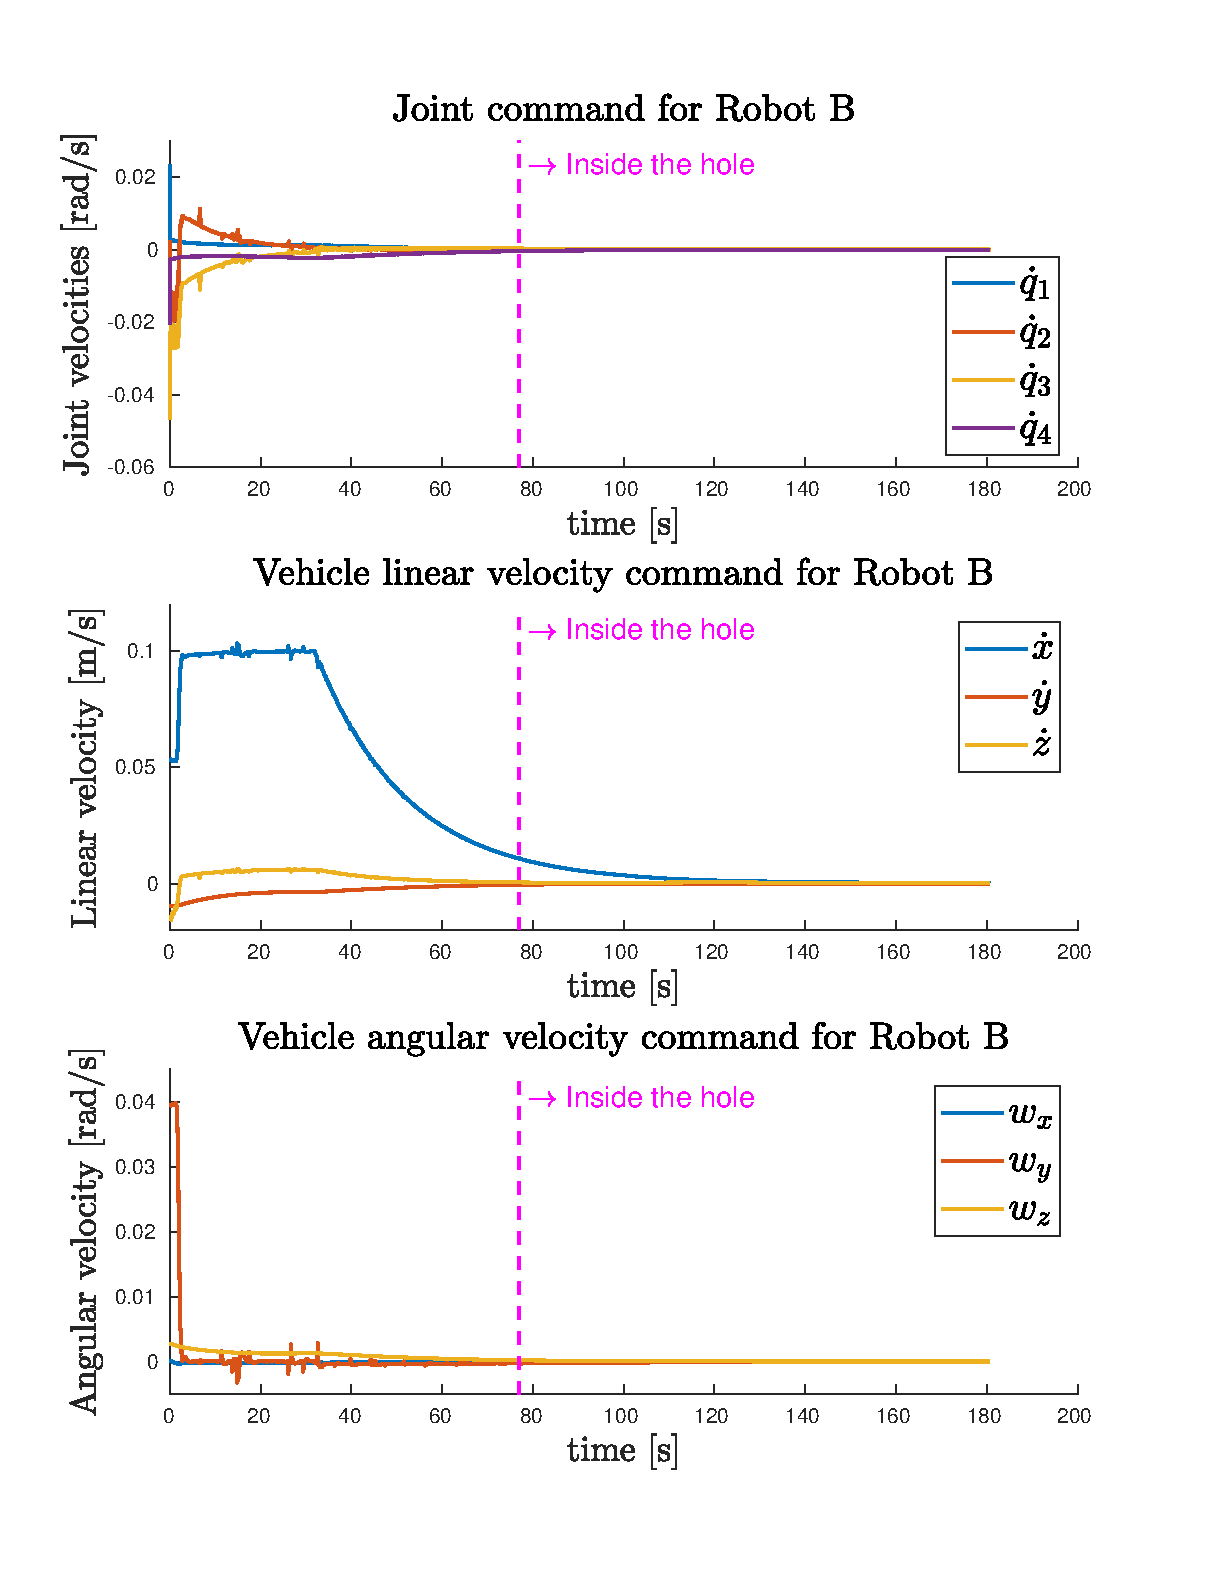
\includegraphics[width=9cm]{withVisio/coopJoinVelB.eps}
	}

	\caption[Plots of cooperative robots velocities]{The system velocities $\dot{\hat{\boldsymbol{y}}}_a$ and $\dot{\hat{\boldsymbol{y}}}_b\,$, outputs of the kinematic layer after the cooperation policy (section \ref{sec:coopScheme}) and the arm-vehicle coordination scheme (section \ref{sec:armVehScheme}). These are not always the \emph{real} robot velocities because they do not include velocities caused by collisions (for robot A) and by firm grasp constraint (for robot B).}
	\label{fig:expWithVisioVel}
\end{figure}

\begin{figure}[H]
	%todo metti inside the hole vertical bar
	\centering
	\textbf{Results with hole's pose estimation by Vision}\\
	\textbf{Cooperative tool velocity (after cooperation)}
	\vspace{20px}
	\centerline{
		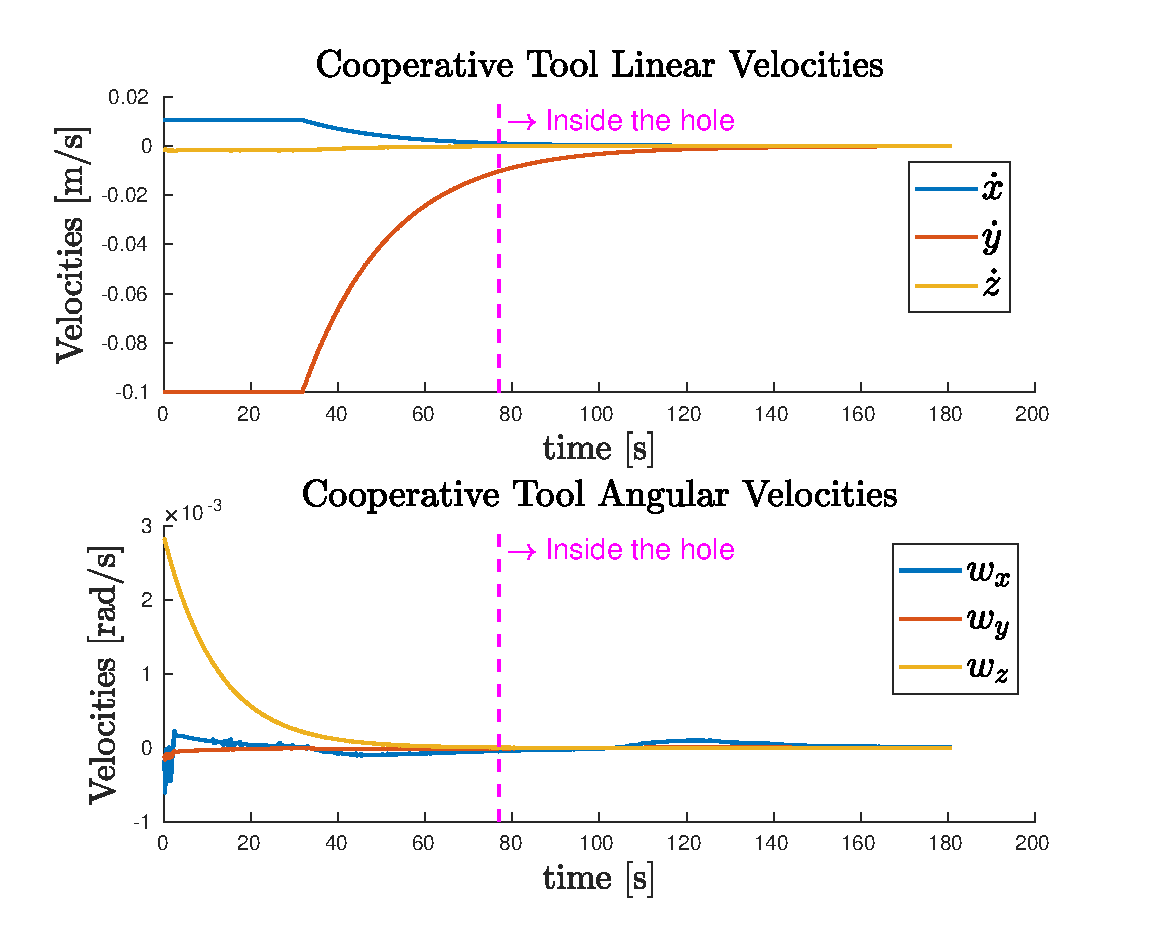
\includegraphics[width=12.5cm]{withVisio/coopToolVel.eps}
	}
	\caption[Plots of cooperative tool velocity]{The tool velocity $\dot{\tilde{\boldsymbol{x}}}_t$, the one that the coordinator sends to both robots during the coordination policy. It is the \emph{feasible} one that \emph{both} robots provide to the tool (section \ref{sec:coopScheme}), and it is caused by the system velocities of figure \ref{fig:expWithVisioVel}. So, it is not always the \emph{real} velocity that the tool has because collisions and firm grasp constraint are not included.}
	\label{fig:expWithVisioVelTool}
\end{figure}



\section{Results Discussion}
In this section, considerations about the results shown in the previous pages are made.\\

When the goal frame is know without error, the results are good even without the Force-Torque objective and the Change Goal routine. This is clearly visible in figure \ref{fig:noErrorPlots}. Despite no presence of errors, some collisions happen anyway. This is due to the fact that the peg is driven  directly toward the goal (inside the hole), without considering that there is the hole structure. Anyway, the forces and torques acting on the peg \enquote{help} the insertion phase because they drive \textit{naturally} the tool inside the hole. The peaks of the magnitudes are due to the first contact with the hole: even if the pose is perfect, this does not mean that a perfect alignment is present \textit{before} reaching the goal frame.
The lower left plot of figure \ref{fig:noErrorPlots} shows the tool velocities caused by the collisions, and in the lower right one we can see that the second tool \enquote{follow} the velocities of the first one, due to the firm grasp constraint (around second 40). In other words, it is as if the robot B would be dragged by motions causes by collisions on robot A. In the same plot, the chaotic velocities caused at the beginning are due to a not-perfectly coincident initial position of the two tools, that is impossible to achieve due to numerical errors of the simulation. Anyway, after a while they go to zero, so this initial error does not affect the rest of the experiment.\\ 
The upper right plot shows how the error converges along its components. The small peak in roll is caused by the initial collisions with the hole.\\
Even if a perfect goal pose is obviously impossible to have, this experiment is useful to understand how the peg is inserted if ideal conditions are present. This is important: from now we know that in any case, the forces and torques acting on the peg may help \textit{naturally} the insertion phase.\\

% confronto change goal vs no change goal
When an error in the goal pose is present, the results obviously get worse. The first noticeable thing is in figure \ref{fig:comparison_final}: due to the error the collisions are more present during the insertion (first plot). An interesting thing is that the peg is inserted at the wanted depth anyway (as can be seen in the right lower plot, where the norm converges to a small value). An issue is that the forces are not nullified at the end, which means that continuous pressure between the peg and the hole is present.\\
The first idea to reduce the number of the collisions is to introduce the routine which change the goal frame. From the plots in the middle of figure \ref{fig:comparison_final}, we see that the overall behaviour is improved: the forces and torques have a littler norm in general (upper plot) and the final position of the tool is more precise (lower plot). In fact, from figure \ref{fig:Error_nothingandgoal_plot6} the six lower plots show us that the error in $x$ is corrected by the routine. It can be noticed that also the $z$ component is modified, even if it has no initial error. This is caused by the fact that the routine is active: so all the components are modified in the direction of the detected forces. Obviously, we can't assume to have an error only along a single axis, so we can't modify only the axis where we know there is the error ($x$-axis in this case). In truth, also the \mbox{$y$-component} is modified, even if the change is very little because the component of the force acting along the length of the peg is neglected to not modify the wanted depth of insertion (as explained in \ref{sec:changeGoal}).\\
From the same figure \ref{fig:Error_nothingandgoal_plot6}, another thing to notice is that the routine does not correct perfectly the error in all the components, in fact the goal along the z-component is a bit erroneous. This is because the peg has reached a point where the forces are zero, and so no more modifications can be done. This is caused by the fact that the peg has a smaller diameter than the hole, and so there is a tiny tolerance zone inside the hole where collisions do not happen.\\

%force task

In general, the goal changes slowly: this means that, especially when the first contact happens, the forces and torques magnitudes are big as in the vanilla case. The Force-Torque objective helps to reduce these peaks: as soon as a force (or torque) is detected, the objective responds to it and generates a reference velocity that moves the peg away from the walls of the hole. The reduction of the magnitudes is visible in the third plot of figure \ref{fig:comparison_final}. \\
In the lower plots of the same figure \ref{fig:comparison_final}, it is shown that the positional error between the goal and the tool is not affected so much by this objective. In truth, the convergence of the norm to a small value is a bit slower than the one of the case where this objective is not used. The first factor is that now the collisions are considered by the kinematic layer. So, being the new objective at an higher priority respect to the reaching goal objective, the kinematic control tends \textit{first} to nullify the forces and torques and \textit{then} to drive the tool toward the goal. This, sometimes, could increase the time to accomplish the mission (as in this case). Anyway, some other times it can \textit{decrease} the mission time because less stalemates happen, thanks to the fact that this objective may help drive the peg away from the collision. In the second plot of figure \ref{fig:comparison_final}, we can see that the norm of the force stays at almost a constant value around the interval $80s-180s$, as well as the norm of the error in the plot below. This shows a situation of stalemate that is then solved. Presence of standoffs like this one are discussed later. A second factor is simply that, being the particularity of the problem, each experiment is different from the others, so sometimes the mission is \enquote{lucky} and it has less difficulties.\\
Figure \ref{fig:forceTaskActRef} shows how the new introduced objective generates references and activations in correspondence of the forces and the torques detected: obviously the references and activations shapes (lower four plots) are similar to the shape of the forces and of the torques (depicted in the two upper plots). In this case they are even more similar because the norm (which is the quantity that the objective controls) is given by almost only one component, the $y$ one.\\ 
In the lower plots, the activation is a function which assumes only values from $0$ to $1$, so it is always positive. The references instead, have opposite sign respect to the forces and the torques. This is because the objective wants to \textit{nullify} the forces and the torques, so it provides a velocity in the opposite direction.\\ 
In the reported plots reference and activation are the ones calculated by robot A, but for the robot B they are the same. The agents receive the same data from the sensor (except small synchronization problems that can happen), so the reference $\dot{\bar{\boldsymbol{x}}}_{ft}$ and the activation 	$\boldsymbol{A}_{ft}$ are the same.\\

Figure \ref{fig:forceTaskVelocities} shows the results of $\; \boldsymbol{J}^{\#}_{ft} \; \dot{\bar{\boldsymbol{x}}}_{ft}\;$, for both robots. These are the system velocities that we would give if the objective was the only one in the TPIK list, without considering the activation, and a simple pseudoinverse for the Jacobian was used (without any regularization). So neither the collision propagation, the firm grasp constraint, nor the cooperation are included. As explained before, the reference $\dot{\bar{\boldsymbol{x}}}_{ft}$ is the same vector for both agents. The thing that makes the two velocities so dissimilar, is the Jacobian $\boldsymbol{J}^{\#}_{ft}\,$, which is obviously different for each agent because they have different poses. This difference, at this point, it is not a problem for the cooperation because we have still to deal with the coordination policy.\\
These plots are shown only to point out that the velocities are not so big to be not feasible. In truth, at least for the vehicle part, they could be even too small to be followed well. This can be solved to make the objective control only the arm, or by increasing the gains (but taking into account that bigger gains would mean bigger risks of bad behaviours). Another thing we can see is that they are not so smooth, and they have lot of fast changes. However, firstly we have to consider that the activation, which the main work is to smooth the behaviour, are not present. Then, magnitudes are so little (in the $0.01rad/s$ order for joints, and in the $0.01m/s$ and $0.04rad/s$ order for vehicle) that these fast changes are not so important. Last, we can't do so much because these changes are given by external data (the forces and the torques) that we have to deal with.\\

The final test of section \ref{sec:finalTest} (which includes the Vision part) is interesting for two main reasons. The first one is that the peg does not start so near the hole (but it is almost aligned to it as before). This shows that the transportation phase is done in a good manner by the cooperative robots, even if no difficulties (e.g. difficult trajectories, an obstacle, a joint limit, and no vehicle and arm dynamics) are encountered.
The second reason is that here we have hole's pose error also with some angular component, that affect the orientation of the goal frame where the peg is driven to. Anyway, this error is small and do not influence too much the insertion. In fact, as we can see in figure \ref{fig:expWithVisio}, the norm of the forces and of the torques is smaller than previous (upper left plot); the error converge smoothly (upper right plot); and little modifications are done to the frame goal, because its origin is almost with no error (lower plots). The bigger error in the angular norm is obviously due to the fact that now there are also some imprecisions in the orientation of the hole.\\

Figure \ref{fig:expWithVisioVel} shows some plots about the cooperation. No big difficulties are met by the robot during the transportation and the insertion. So, the system velocities, that are the outputs of the final TPIK procedure (after the cooperation policy and the arm-vehicle coordination), are similar between the two robots. It must be remembered that these velocities are not the applied one because the disturbances caused by collisions and firm grasp are not included. However, for the robot B (right plot) we can see that tiny peaks are present around the interval $20s - 40s$. These can be caused \textit{indirectly} by the firm grasp constraint. When the tool of robot B is driven away a bit, in the next control loop the kinematic layer must do a little more effort in recovering the trajectory, causing these tiny peaks. Being the cooperation policy included, if these peaks are high (as around second $8$) the Robot A helps the other one, in fact a little peak is present also for this one.\\
The last figure \ref{fig:expWithVisioVelTool} shows the \textit{feasible} \textit{cooperative} tool velocity $\dot{\tilde{\boldsymbol{x}}}_t$, that is the one that the coordinator sends to the two agents, after assuring that is achievable by both (as explained in section \ref{sec:coopScheme}). Even if disturbances of collisions and of firm grasp constraint are not present, this plot gives an idea about the tool's speed during the mission. It is driven slowly because the problem needs so: the insertion phase, made by two kinematic cooperative manipulators, puts big challenges and we can't afford to have too big gains.\\

A last thing to report is that some experiments meet a standoff situation at some point during the insertion. This happen when the collisions continuously make the peg to \enquote{bounce} on the inner hole walls, making it moving back and forth. The \enquote{bounce} is due to a bad peg alignment inside the hole, so the tip continuously touches the inner wall. In these cases, sometimes, the methods used do not manage to solve the stalemate in a reasonable time. The problem can be due to different factors. One could be that the simulation, being only kinematic, is not precise. So, even if the gain are really small, in any case the velocities are instantaneously provided to the system, and this causes always a bit chattering. This complicates the work of the simulator (to calculate the collisions) and of the whole mission (that could meet almost instantaneously a strong force or torque). Another problem could be a not so good setting of the many gains that we have to put. Other one can be that we have two robots that are carrying the peg, which makes the whole experiment much more difficult, considering also that the collisions propagate through Jacobians (that are mappings from linear approximations of non-linear things) on the system. Other one can be that, with the Change Goal routine, orientation modifications are not made, so no correction is doable for the angular part. Additional issue to take into account is that some synchronization issues may happen. The coordination policy, in the way it is implemented, assures the synchronization (section \ref{sec:controlLoop}), but we have also other kinds of exchanged information. For example, the force-torque sensor data is shared using ROS topics in a simple way, so with the actual software we can't know exactly when information arrives to each node. Considering also that on a single machine we run the simulation and the two robot software (plus the coordinator) this could cause more synchronization problem. This may be solved with further code improvement, but it goes out of the scope of this work and it is not so useful for the real application (where we don't run everything on a single machine).\\
The standoff problem is more influential when the hole's pose error is bigger, or, for example, when we have also orientation error such as in the last experiment. However, the methods show a good starting point to improve the current state of art in this unexplored problem underwater.
